%!TEX TS-program = xelatex
%!TEX encoding = UTF-8 Unicode

\documentclass[School=EMC]{Dissertate}
\usepackage{tikz}
\usepackage{chapterbib}
\usepackage{natbib}

\begin{document}

% the front matter
\begin{titlepage}
%\usepackage{tikz}
\tikz[remember picture,overlay] \node[opacity=0.5,inner sep=0pt] at (current page.center){\includegraphics[width=\paperwidth,height=\paperheight]{frontmatter/images/cover.jpg}};
%\clearpage

\begin{center}

\color{emc-dark-blue}{
\vspace{-2cm}
\huge{
    \sc{
    \textbf{ \uppercase{The Jigsaw Genome}} \\
    some clever subtitle}

    \vspace{16cm}

    \LARGE Saskia Hiltemann}
}


\begin{comment}
\newpage
real jigsaw out of image: http://www.jigsawplanet.com
make my own jigsaw puzzle cover image: http://www.photoshopessentials.com/photo-effects/photoshop-puzzle/

\includegraphics[width=8cm]{frontmatter/images/jigsaw_genome2.jpg}

\includegraphics[width=8cm]{frontmatter/images/jigsaw_genome1.jpg}

\includegraphics[width=8cm]{frontmatter/images/jigsaw_genome3.jpg}
\end{comment}
\end{center}
\end{titlepage}

% Some details about the dissertation.
\title{Bioinformatics for Everyone}
\author{Saskia Hiltemann}
\advisor{Bigname Scientist}

% ... about the degree.
\degree{Doctor of Philosophy}
\field{Bioinformatics}
\degreeyear{2024}
\degreemonth{May}
\department{Bioinformatics}

% ... about the candidate's previous degrees.
\pdOneName{B.S.}
\pdOneSchool{Boston University}
\pdOneYear{2018}

\pdTwoName{M.A.}
\pdTwoSchool{Monster's Univeristy}
\pdTwoYear{2021}

\maketitle
\copyrightpage
%\abstractpage
\dedicationpage

% the abstract
\chapter*{Foreword}
\setlength\parindent{0pt}
\vspace{-1cm}
The big red button. In every bioinformatics-oriented presentation my supervisor gave over the years of my PhD studentship this familiar slide reappeared.
It is the biologist's dream; a mythical and mystical red button that takes their raw data and transforms it magically into a \emph{Nature} paper ready for submission.


Of course this is an unattainable dream, but there are many steps we can take to easy the burden of data analysis and decrease the
turnaround time between sample collection and manuscript submission. 

\chapter*{Stellingen}

Eleven propositions must be added to the doctoral dissertation. Of these propositions,
five must relate to the contents of the doctoral dissertation and five must not relate,
either directly or indirectly, to the contents of the doctoral dissertation. These ten
propositions must be academically defensible. The eleventh proposition does not have
to meet the criterion of academic defensibility. The doctoral candidate must submit the
propositions to the doctoral dissertation supervisor as soon as possible following the
approval of the doctoral dissertation as referred to in Article 5.1.

\begin{itemize}
\item 5 from thesis, academically defensible
\item 5 unrelated to thesis, academically defensible
\item anything, academically defensible or not
\end{itemize}

\chapter*{Structure of Thesis}
\vspace{-2cm}
(TODO: remove, this is just a note for myself/reviewers)


\textbf{Title: } Bioinformatics for Everybody \\
\textit{Reasoning: }\vspace{-1.8em}
\begin{itemize}
\itemsep-0.5em
  \item \textbf{Galaxy:} empowers researchers to run their own analyses
  \item \textbf{Training materials infrastructure:} educates researchers to understand their own analyses
  \item \textbf{Visualisation and reporting:} for easy interpretation of results (e.g. for clinicians)
\end{itemize}
\vspace{-1.8em}
Focus on accessible, reproducible, user-friendly bioinformatics and open science principles.


\textbf{Publications:} \\

Chapter 1-3: The bioinformatics foundations \\
Chapters 4-6: Use cases; split into "the bio" and "the informatics"; Technical paper \& the biological insight it led to/facilitated \\

\begin{itemize}
\itemsep-0.5em
\item \textbf{Chapter 1:} Galaxy platform \\
\item \textbf{Chapter 2:} Training Materials infrastructure paper \\
\item \textbf{Chapter 3:} Visualization \& results reporting \\
  - iReport paper \\
  - Circos paper (hopefully)
\item \textbf{Chapter 4:} Use case: Fusion Gene Detection \\
  - the informatics: iFUSE paper \\
  - the bio: VCaP chromothripsis paper
\item \textbf{Chapter 5:} Use case: Somatic Variant Detection \\
  - the informatics: CGtag paper (Galaxy tool suite) \\
  - the bio: Virtual normal paper
\item \textbf{Chapter 6:} Use case: Micriobiota Profiling \\
  - the informatics: GmT paper (Galaxy tool suite \& training manual) \\
  - the bio: MYcrobiota platform
\end{itemize}

\textbf{Structure of Introduction}

\begin{itemize}
\item \textbf{The Source code of life} - General introduction to DNA and backgrund on genome sequencing
\item \textbf{The Bioinformatics Challenge} - Some challenges faced in bioinformatics analyses
\item \textbf{Bioinformatics Best Practices} - Some guidelines for high-quality bioinformatics tools and practices to help deal with challenges mentioned in previous paragraph
\item \textbf{Bioinformatics for Everybody} - Galaxy and Training materials as key component for delivering accessible, user-friendly bioinformatics analyses for non-bioinformaticians
\item \textbf{Use Case 1: Prostate Cancer} - Cancers complexities (Fusion genes, chromothripsis), somatic variant detection
\item \textbf{Use Case 2: Micriobiota profiling} - Intro to the microbiome, 16S rRNA sequencing vs whole-genome shotgun
\end{itemize}

\textbf{Structure of Discussion}

\begin{itemize}
\item \textbf{TODO}
\end{itemize}


\tableofcontents
%\authorlist
%\listoffigures

\abstractpage
%\doublespacing

% include each chapter...
\setcounter{chapter}{-1}  % start chapter numbering at 0 because (computer) science
\chapter{Introduction}
\label{introduction}
 % start numberings at 0 because (computer) science
\setcounter{figure}{-1}
\setcounter{table}{-1}
\setcounter{section}{-1}
\setcounter{NAT@ctr}{-1}

\setlength\parindent{0pt}

\section*{Contents}

\begin{enumerate}
\itemsep-0.5em
\item A Brief History of Genomics
\item A Primer on Sequencing (?)
\item The Bioinformatics Challenge
\item Bioinformatics Best Practices
\item The Galaxy Platform
\item Use case 1: Prostate Cancer
\item Use case 2: Microbiota Analysis
\item Scope of this Thesis.
\end{enumerate}

\section{A Brief History of Genomics}

\begin{comment}
Set the stage, lots of data being generated, need to keep up on the analysis side as well.

- More specifically mention 1st generation, next gen, 3rd gen
\end{comment}

DNA. The blueprint of life. These long double-stranded helical molecules are present in all living cells on earth\footnote{As far as currently known. Some viruses contain only RNA, but these are often not considered "alive".} and encode the proteins which drive the functioning, regulation, structure and replication of the cells and tissues that make up an organism.

\subsection{The Source code of Life}
Any computer program, no matter how complex, can be described as a long series of just two characters, `0` and `1`, known as \emph{bits}. However, knowing the sequence of bits alone is not enough to understand what these programs do; for this we also need to know the details about how they are being interpreted by the machine on which they are executed. In much the same way, DNA uses just 4 different elements, called \emph{bases} or \emph{nucleotides}, to encode its blueprint for the cell. These 4 building blocks are adenine, cytosine, guanine and thymine, usually referred to simply by their first letters, `A` `C` `T` and `G`. These bases combine together in pairs (\emph{"base pairs"}), with `A` matching to `T` and `C` mathing to `G` in the double-strand helix configuration \ref{fig:dnastructure}.

\begin{figure}[h!]
    \centering
    \includegraphics[width=300pt]{chapters/images/introduction/dna-structure.jpeg}
    \caption{Structure of DNA}
    \label{fig:dnastructure}
\end{figure}


\subsection{Sequencing}
In 1990, the Human Genome Project \cite{olson1993human} set out to sequence the entire 3.2-billion-basepair-long human genome, an effort culminating in 2003 with the publication of the first human \textit{reference genome} \cite{international2004finishing}. Not only did this provide invaluable insights into human genetics, but it also paved the way for the next era in genetic research; something which would completely transform the field of genetic research. Over the next several years, next-generation massively parallel sequencers were developed by companies like Roche454 and Illumina, dramatically cutting the cost and time required to sequence a human genome, and for the first time demonstrated its potential utility in clinical and diagnostic settings. Through sustained technological advancements over the following years, these costs continued to decrease at exponential rates - outstripping even the pace predicted by Moore's law (\hyperref[fig:seqcost]{Fig. \ref{fig:seqcost}}) - and the long dreamed-about \textit{\$1,000 dollar genome} \cite{thousanddollargenome} \cite{sequencingcostsNHGRI} has now become a reality.

\begin{figure}[h!]
    \centering
    \includegraphics[width=300pt]{chapters/images/Historic_cost_of_sequencing_a_human_genome.png}
    \caption{The cost of sequencing a human-sized genome over time. Data from the NHGRI Genome Sequencing Program (GSP) }
    \label{fig:seqcost}
\end{figure}

But DNA is only one part of the story. Shortly after the publication of the human genome, high-throughput techniques emerged to also sequence the transcriptome (RNA-Seq), allowing for the identification and quantification of gene transcripts, and providing information about post-transcriptional mutations and other complexities such as alternative splicing \cite{wang2009rna}. Similarly, the study of epigenetics is revealing that non-coding DNA, far from the once-termed \textit{"junk DNA"}, is part of an intricate and complex regulatory system controlling the expression of genes \cite{zuckerkandl2007combinatorial}.

And now we are now moving into the era of third-generation sequencing, where single-cell \cite{gawad2016single}, long-read \cite{koren2015one}, and often real-time sequencing \cite{flusberg2010direct} are allowing for ever more accurate determination of nucleotide sequence, providing increased resolution even in highly diverse and complex samples such as tumours or metagenomic samples. All these technological advances have led to a deluge of data that must be managed and analysed, typically by bioinformaticians.


\section{The Bioinformatics Challenge}

With huge amounts of data now being generated at relatively low cost \cite{chen2014big}, and compute resources being available even on moderate budgets, the challenge in genomic research has shifted from the sequencing technologies, to the analysis and interpretation of these big and highly complex datasets, and the development of the software required to do so, in order to gain new understanding of the underlying biological systems. This poses a significant challenge, both technologically and scientifically.

\subsection{Ever-changing landscape}
Sequencing technologies are evolving at a staggering pace, and with them so must the software tools necessary to analyse and understand the data. Therefore, new tools are developed continually and existing tools must be updated regularly to remain relevant. As a consequence, there typically simply is not enough time for community standards and consensus pipelines to emerge organically before new technologies make them obsolete. Because of this, there usually are a multitude of tools available for any given task, each with their own set of advantages and disadvantages, and the challenge is to find the right tool for your particular situation, and knowing when to use existing tools and when the development of novel tools is in order.

\subsection{Standardisation}
Such a lack of clear standards does not only apply to software tools, but also to file formats, and this poses a major hurdle in data analysis. While some clear data format standards exist [fastq, VCF], there are many cases that lack such a standard, hindering the interoperability of different tools. And even the more established file formats such as fastq and VCF allow for a variety of flavours, e.g. different fastq quality encoding schemes, which are not indicated inside the file format specification itself, but may influence downstream results. Thus, when creating analysis pipelines from existing tools, many file transformation steps are typically required as a kind of \textit{glue} between steps.

\subsection{Data Storage}
 \begin{comment} https://qumulo.com/blog/genomic-sequencing-qf2-storage/ \end{comment}
Sequencing data is being generate at a rate of X petabytes per year (TODO: find citation), and all this data must be stored somewhere. But there is more to data storage than buying a hard disk and copying data. The data must be backed up to prevent data loss, it must be made available for use in an efficient way (I/O matters), data must be organised and tracked in a usable manner, and any solution must be able to scale to the exponential trend of growth both in size and number of files generated. Furthermore, data storage must comply with privacy and security requirements, especially important in the case of human genetic data.


\subsection{The Specialist Bioinformatician}
All of these challenges have resulted in bioinformatics becoming a highly specialized field, which in itself poses a new challenge given the observation that the domain knowledge (biology) and the informatics know-how more and more often do not reside in a single individual, and the interpretation of the data cannot always be done by the person performing the data analysis and vice versa. Instead, close communication between the two fields is required, and the domain experts should be empowered to perform their own data analyses as much as possible.

\verb+informatician needs to shine a light in the black box that is the wetlab, domain expert needs to become comfortable with the informatics, since this has become an integral part of any analysis+


% some (partial) solutions to the above challenges, spoilers: open software, open science, open everything
\section{Bioinformatics Best Practices}
Since bioinformaticians are primarily academics -who are typically being judged on their publications, not their code-, the quality of bioinformatics tools is highly variable and tool authors often struggle to find the time and resources to maintain their code. The open-source community is instrumental in this respect, allowing the most popular and useful tools to be taken up by the community which can collectively maintain and update the bioinformatics software packages. Adhering to a set of best-practices guidelines can greatly reduce this maintenance burden, and increase the chance of tools being taken up by the community.

Many journals require authors to submit datasets to public repositories in order to allow other scientists to reproduce their findings. With bioinformatics now such a fundamental part of any publication, a clear description of the analysis pipeline is also required for true reproducibility, but the majority of scientific publication do not contain all the information required to reproduce the in-silico experiment [cite]. Making analysis software open-source and adhering to a set of bioinformatics best-practices can improve the reproducibility of bioinformatics analysis pipelines.

Such bioinformatics best-practices include:

\begin{enumerate}
    \itemsep-0.5em
    \item Accessibility of tools and data %(usability) of tools (documentation, open source, github etc, galaxy, galaxy, dependency management, docker)
    \item Reproducibility %(conda, docker, galaxy, version control, code notebooks)
    \item Interoperability %(data formats, common frameworks, generic, allow for packaging)
    \item Maintainability of software %(testing, continuous integration, community buildingi, scalability)
    \item Visualization and reporting
    %\item Data management and sharing %(FAIR data, LIMS, PIDs)
\end{enumerate}


\subsubsection{Accessibility}
Most bioinformatics tools are commandline unix tools, and biologists are not typically trained in the use of such. Even for the experienced bioinformatician, running some of these tools can be a challenge due to lack of documentation or quality of the tool. Ideally, once a tool or pipeline has been validated, the analysis can be run by the domain expert, i.e. the research scientist responsible for the interpretation of the analysis results, without being reliant on the support of a bioinformatician at every step \cite{kumar2007bioinformatics}.

Creating user-friendly software is not a trivial task. Application linking (also referred to as wrapping), can ease this burden for the tool developer. In such an approach, existing user-friendly interfaces host third-party software packages -at miniumum effort to the developer of the hosted software- and thereby offer a layer of abstraction to the end-user that shields them from the implementation details of the tool and provides a uniform usage paradigm for all tools, regardless of their differences behind the scenes. Examples of such hosting frameworks in the context of bioinformatics are Galaxy \cite{giardine2005galaxy,goecks2010galaxy}, Taverna \cite{}, [more?].

Accessibility also includes high-quality documentation of the tool, both for developers and end-users, and ideally some form of training manual to educate users in the proper use of tool and warn about possible pitfalls and biases.

\subsubsection{Reproducibility}

A cornerstone of the scientific method is reproducibility of results. Experiments should be described in sufficient detail to allow for their reproduction and independent verification by fellow scientists. In reality however, this remains a big challenge, and many publications can not be reliably reproduced based on the information provided in publication []. In many cases this holds not only for the wetlab experiment, but also for the in-silico downstream data analysis. Reproducing bioinformatics analyses often becomes an exercise in \textit{"forensic bioinformatics"}; trying to piece together the exact procedure used through trial and error and educated guessing. In part this is caused by journals not having clear submission guidelines for bioinformatics pipeline description as they do for the physical samples. The latter are commonly required to be submitted to biobanks before submission, and the raw datasets generated from them to be stored in online repositories. No such requirements are generally imposed on the downstream analysis, or when they are these requirements are not strict enough to ensure true reproducibility. This is not without consequences; in some cases this has lead to clinical trials being started based on incorrect conclusions not revealed during peer review due to lack of reproducibility \cite{baggerly2009reproducible}.

% dependency management
But even if the full source code were made available, reproducibility of the entire dependency chain of all software and system libraries used remains problematic. Every package in this dependency tree has the potential to influence the final result. While reproducibility is a high priority in the scientific community, this isn't the same for software developers in general, and many packages will simply be removed when an update has been made available. This is where package managers such as Conda \cite{gruning2017bioconda} or GNU Guix \cite{courtes2013functional} offer significant improvement, by allowing specific versions of tools to be installed, and mandating that any changes made to a package must be submitted as a new version, and existing version remain available and unchanged indefinitely. This ensures that the stack of software obtained when installing a tool at a specific version will yield identical results today as it will a year from now.

% provenance
Once the correct set of software is obtained, the provenance of how the tools were applied to the data must also be logged. This includes the sequence and interplay of different tool executions, with the full parameter settings and input and reference data used at every step. Keeping a lab journal of the in-silico experiment is a good start, but too error-prone as a manual process. Projects such as Jupyter Notebooks \cite{kluyver2016jupyter} for Python, or Sweave \cite{leisch2002sweave} and KnitR \cite{xie2014knitr} for R, allow for the mixing of text and tools to create interactive journal articles if you will, where the calculations are embedded within the manuscript, and these calculations can be examined and rerun or adjusted with ease. A drawback of this of course comes when tools require a lot of resources or are not all written in the same language, as is typically the case for NGS analyses. Workflow platforms such as Galaxy \cite{} automatically keep track of provenance for the user and have the advantage of supporting a wide range of tools.


\begin{comment}
"forensic bioinformatics" -> have to figure out by trial and error what was done

https://bmcmedresmethodol.biomedcentral.com/articles/10.1186/s12874-017-0377-6
https://www.biostars.org/p/52561/
https://www.nature.com/naturejobs/science/articles/10.1038/nj7396-137a
https://www.nature.com/nm/journal/v13/n11/full/nm1107-1276b.html
\end{comment}

\subsection{Interoperability}

A plethora of bioinformatics tools are available, and most analyses require combining a number of tools together into an analysis pipeline, also referred to as a workflow. The different components in such a pipeline usually do not work seamlessly together without a bit of "glue"; custom scripts that convert the output of one tool so that it can be used as input for the next. This is necessary due to the frequent lack of clear data formats. For example for structural variations, no clear data format exists, and most tools output custom formats. Many of these custom formats contain the same information, it is often formatted differently. Any tools working on such datasets make assumptions about its format, so we must take care to adhere to these expectations. Even in cases where file formats are more standardized, variations in the exact implementations may still require careful consideration within a pipeline. Consider for example the fastq format; this is a relatively simple format, just 4 lines per sequence read, but the fourth line, the line containing quality score, is the source of some divergence in the format. A range of ASCII characters is used to encode numerical values indicating a PHRED-like quality score of the base call, but the range and start position of this character range comes in different flavours. Furthermore, because these ranges overlap, it is not always possible to deduce which convention was used unless some quality encoding are present in the file that only appear in one of the conventions. It is therefore important to know the convention used for any datasets entering your pipeline, and know when tools make assumptions about their input data. If necessary, a format conversion step can be employed to resolve any mismatches between the format expected by a tool and the format of the input dataset. Similar widespread variations in standard formats include chromosomal location (0-based or 1-based numbering, open or closed) and chromosome names (with or without a `chr` prefix). These issues are not hard to deal with, but can lead to inaccurate results if not carefully taken into account by the creator of the pipeline.

% packaging
On a more technical level, different tools may be written in different programming languages and/or compiled for different operating systems, and it can be a challenge to combine these into a single analysis. Luckily, tool developers can undertake steps to make their tools more interoperable. Package managers such as bioconda will compile software from its source for different operating systems. For bash scripts, many OS-dependent syntax variations can hinder interoperabililty, but by taking care to comply with POSIX standards, such concerns can be mitigated. Vitally, precise documentation of any assumptions made in the code is indespensible, and making source code open further facilitates this transparancy.


\begin{comment}
file format standards, common frameworks, good documentation, open-source,
allow for packaging (don't deliver code as VMs etc),
\end{comment}

\subsection{Maintainability}
In bioinformatics, the emphasis for scientific accomplishments is placed on scientific publications, not on software products. As a result, many tool developers struggle to find the time and resources to maintain their software beyond its release. Since scientific research depends increasingly on these pieces of software, decreasing the burden of tool maintainence is valuable and worthwhile pursuit. Furthermore, many tools are written by small research groups or single individuals who are simply unable to perform the necessary maintainence without support. By making tools open-source, the entire bioinformatics community is able to step up as co-developer, allowing them to discover bugs and contribute fixes or enhancements. Code sharing platforms like GitHub \cite{} and BitBucket \cite{} facilitate this community-driven approach to software maintainance.

Using code versioning such frameworks such as git \cite{} or mercurial \cite{} ensures precise tracking of changes and ability to revert to any previous state at minimal effort, and facilitates merging of that Incorporating tests at every phase of development can further decrease the maintenance effort. Unit tests ensure that small code modules show expected behaviour at all times. Functional tests ensure that these different units of code always yield the desired result when working in conjunction. Code quality checks can help streamline the code itself and increase readability, benefiting future development. Continuous integration is the paradigm whereby changes to the mainline code are incorporated incrementally and continually, and thoroughly reviewed and tested at every stage.

%versioning continuous integration, functional testing, code review, dependency resolution (conda)

\subsection{Visualisation and Reporting}

As scientists become increasingly reliant on large and complex computational analyses in their research \cite{chen2014big}, the final analysis result datasets become similarly complex and have  often grown beyond the realm of what can be manually viewed and interpreted, both in terms of the number of files and their sizes, as in terms of complexity. Analysis results therefore require summation and visualisation and must be presented to the domain expert in a comprehensible and accesible manner. Such a report should also contain detailed descriptions of the methods used and assumptions made and citations to any third-party tools employed, as an understanding of these factor can assist in interpretation \cite{kumar2007bioinformatics}.

For genomics data, visualisation tools such as Circos \cite{circos} [list more examples] enable the integration of various output datasets, often in the order of millions of lines each, to be summarized in a single image. While some resolution may be lost in such visualisations, they do enable the easy identification of areas of interest and guide the interpretation by pointing the domain experts in the direction of further inspection.


\section{The Galaxy Project}
The Galaxy project \cite{afgan2016galaxy} facilitates many of the best-practice bioinformatics guidelines outlined in the previous section. Galaxy provides a graphical web-based interface to commandline bioinformatics tools, bringing the data analysis to the domain experts equipped to perform the interpretation of the results. With its heavy focus on accessibility and reproducibility, Galaxy is an important component in creating high-quality bioinformatics pipelines. Galaxy keeps track of the full analysis provenance, manages tool dependencies with bioconda \cite{}, has built-in visualisations, and is accesible by end users with nothing more than a browser. For developers, Galaxy provides a convenient framework to package tools to make these available for researches throughout the global community. The Galaxy toolshed

\section{Training}
With -omics research becoming increasingly computational in nature, and many research groups not having access to a dedicated bioinformatician, there is a great need for high-quality bioinformatics training to ensure that the domain experts who interpret the results of data analyses are optimally equipped to do so. Surveys confirm this need for bioinformatic training; the majority of researchers (>95\%) work with or plan to work with large datasets, but most (>65\%) possess only minimal bioinformatics skills and are not comfortable with statistical analyses \cite{larcombe2017elixir}, \cite{williams2017vision}. Demand for training currently greatly exceeds the supply \cite{attwood2017global}. In a recent survey \cite{survey2013embl} over 60\% of biologists expressed a need for more training while only 5\% called for more computing power. Thus one can assume that the true bottleneck of the current data deluge is not storage or processing power, but the knowledge and skills to utilize existing resources.

With its focus on accessibility and user-friendliness, the Galaxy platform is also an ideal environment for teaching. Trainees are shielded from the minutia of the implementation details of the underlying tools, and need nothing more than a browser to execute the tutorials. Because Galaxy can host any commandline tools and the tools available in the tool shed cover a wide range of topics, creation and maintainence of a set of training materials must be a a community effort, with content being created by a large number of people with expertise in the various topics.

[TODO: slightly plagiarized from my own paper, rephrase?]

\newpage
\thispagestyle{empty}
\begin{center}
\vspace{2cm}
\begin{minipage}{6in}
\tikz[remember picture,overlay]
\node[opacity=0.8,inner sep=0pt] at (current page.center){
    %\includegraphics[width=\paperwidth,height=\paperheight]{chapters/images/background-texture-blue.jpg} %higherquality image but too big for overleaf
    \includegraphics[width=\paperwidth,height=\paperheight]{chapters/images/background-texture-blue-reduced.jpg}
};
\sc
\begin{center}

\color{white}{
\Large Prostate Cancer \normalsize
\vspace{2cm}


I like puzzles. Any type of puzzle. I always have. If I see a puzzle or a problem I have to solve it. I think that is what makes cancer such a fascinating topic for me.

\vspace*{0.5cm}

Imagine you are given a jigsaw puzzle. Now instead of a few hundred pieces, there are several billion pieces. The picture on the box is not a picture of the puzzle inside the box,
it is just a somewhat similar image. Oh, and did I mention there are a whole bunch of pieces missing? and that many pieces are duplicated? Some pieces don't even belong in our box,
but come from a completely different puzzle. On top of that your little sister has spilled paint over some of the pieces so those can't be trusted to contribute to the image. And instead of one
single puzzle, the box contains several, they are all variations of the image on the box, but you have no idea how many different puzzles the box contains. Sound challenging? This is the problem we are solving whenever we sequence a cancer genome.

\vspace*{0.5cm}
\textbf{[Metaphor key]} \\
\textit{puzzle pieces} = sequence reads \\
\textit{picture on box} = reference genome \\
\textit{missing pieces} = hard-to-sequence areas \\
\textit{other puzzles} = contamination \\
\textit{painted pieces} = sequencing errors \\
\textit{multiple puzzles in box} = clonality
}

\end{center}
\end{minipage}
\end{center}



\newpage
\section{Use case 1: Prostate Cancer}

\subsection{Background}
\epigraph{3in}{The time has come in America when the same kind of concentrated effort that split the atom and took man to the moon should be turned toward conquering this dread disease.}{President Richard Nixon}

On December 23, 1971, President Richard Nixon, buoyed by recent technical feats such as the moon landing, signed into law the National Cancer Act, thereby declaring a war on cancer. Today, more than 45 years later, that war is still being waged in full force. While great advancements have been made towards this goal, some of the initial optimism has been quelled by discoveries of the great complexity and heterogeneity underlying cancer.

In 2007, technological advancements enabled cancer researchers to look at the complete set of genes (the \textit{exome}) known at the time, in a set of 22 samples of 2 different tumour types. This brute-force, whole-exome sequencing (WES) method yielded a genomic landscape of \textit{mountains} of frequently mutated genes as well as a large number of \textit{hills} that were mutated at lower frequencies across patients, and highlighted once again the vast heterogeneity of cancer genomes \cite{wood2007genomic}.

Since then, many such WES studies on large cohorts of patients have been conducted \cite{wheeler2013human} and have greatly increased our insight into the mutational landscapes of the different tumor types.

...

Prostate cancer remains one of the most common cancers in men, with an estimated 1 in 7 men being diagnosed with the disease in their lifetime \cite{}[cancer.org]. Prostate tumours are often very slow growing, leading to the observation that most men die \emph{with} prostate cancer, rather than \emph{from} it. Early detection is key in selecting the optimal treatment strategy, but prostate cancer often shows few symptoms in the early stages making this a challenge.

A subset of prostate cancers (x \% [cite]) is of a more aggressive type,


\subsection{The Hallmarks of Cancer}

Tumor cells evolve from normal cells through the acquisition and accumulation of mutations. The human body has mechanisms in place to repair or dispose of damaged cells and to prevent runaway cell division, so in order for a tumour cell to survive and thrive it needs to acquire changes that provide it with advantages for proliferation and evasion of the cell's defense mechanisms. Evidence suggests this transformation from healthy cells into malignant cells follows a strikingly similar path across all different tumour types \cite{}. A cell's acquired abilities that drive tumour progression are know as the \emph{hallmarks of cancer} and consist of the following six characteristics:

\begin{itemize}
    \itemsep-0.5em
    \item self-sufficiency in growth signals
    \item insensitivity to anti-growth signals
    \item evasion of programmed cell death
    \item limitless replicative potential
    \item sustained angiogenesis
    \item tissue invasion and metastasis
\end{itemize}

Each of these steps overcomes one of the body's anti-cancer defense mechanisms. This evolution into malignancy is an almost darwinian process where the mutations acquired are random, but those cells that have gained mutations which are advantageous for survival will be able to replicate and thrive and accumulate further mutations. Distinguishing the mutations that impart a strategic advantage and thereby \emph{drive} a tumour's progression, from the often huge number of less harmful \emph{passenger} mutations accumulated over the lifetime of a cancer cell is no easy task. The optimal course of treatment for a patient often depends on the mutations present and how the cell functions are subsequently impacted by those mutations. However, many different mutations may lead to the same disruptions of key pathways, therefore we must evaluate mutations not just as the DNA level but in the broader context of their functional impact on the cell's internal processes.


\subsection{Cancer's Complexities}

Determining the exact genetic sequence of healthy individuals is already quite a challenging endeavor; trying to extend this to cancer genomes takes this challenge to the extreme. There are several complexities present in cancer geneomes that make accurate determination of the genetic changes and their downstream impacts a difficult task:

\begin{enumerate}
    \itemsep-0.5em
    \item Small variants
    \item Structural variations
    \item Clonality
    \item Temporal Evolution
    \item others? Epigenetics? transcriptome level complexities?
\end{enumerate}

In the following sections we will discuss each of these complexities and explore the biological and informatics challenges posed by them.

\subsubsection{The Bio}
\paragraph{Small variants} comprise the simplest class of mutations; those consisting of alterations of just a handful of bases, for instance the \emph{substitution}, \emph{deletion} or \emph{insertion} of one or more nucleotides.

The impact of such mutations depends on where in the genome they occur. Single nucleotide variants (SNVs) in exonic regions can range from having no effect on the resulting protein (silent) to changing an amino acid in the protein to a different amino acid (missense mutations), to changing a codon into a stop codon (nonsense mutation) which nearly always results in a nonfunctional protein. If this happens in a protein that is vital to the functioning of the cell this can have disastrous consequences <some examples of SNVs causing serious problems/phenotypes> <conserved regions, cell's mechanisms for preventing such fatal flaws>

These simple variations were the first to be extensively studied and found to contribute ..

While variants within the coding sequence are most likely to have an impact on cell health, small variants \emph{outside} the coding sequence can also have drastic impact on health, for example 70\% of melanomas exhibit a point mutation in one of two positions in the promoter region of TERT (Horn et al. 2013; Huang et al. 2013).

\paragraph{Structural variations} are larger-scale mutations, involving rearrangement of segments of DNA of more than roughly 50 bp. These often do not involve the coding sequences directly, and can therefore only observed through whole-genome sequencing. Such structural variations can lead to changes in regulation,

<fusion genes>


\paragraph{Clonality}


\paragraph{Temporal Evolution}
\paragraph{Epigenetics}

\subsubsection{The Informatics}

We know that changes in sequence and structure of DNA contributes to cancer development. But how do we describe these properties? Any two healthy individuals differ greatly in their DNA sequence; it's what makes us us. How to denote these differences is a non-trivial problem, as is determining which of these differences are just part of the natural variation between individuals and which are ones detrimental to our health and functioning.

If you were asked to describe the differences between two Shakespeare plays, how would you go about it? They are made up of the same alphabet, and share many of the same words and even whole sentences, but to list the differences between them can be done in many ways. You could number the words in both books and take note of the ones that are different in each position, but then if you were to take two identical sentences and prefix one with a single extra word, all positions would end up being flagged as different while clearly these sentences are nearly identical. And ..

<note: ditch the book analogy? example shakespearean sentence to illustrate? >

poor concordance between variant callers: https://genomemedicine.biomedcentral.com/articles/10.1186/gm432


Currently variations in DNA are described relative to a \emph{reference genome}; a sequence intended to represent the \emph{average} human genome, which was constructed by taking the most frequently observed nucleotide at any given  position in the genome
<discuss some drawbacks/things to realize: based on relatively small set of samples, not optimally diverse set of individuals>

As we have seen, the choice of software can impact downstream analysis, and variant calling is no exception. Different aligners employ different mapping strategies, which leads to different variant calls for the same observed sequence depending on the choice of algorithm, complicating variant comparisons between studies \cite{zook2014integrating}. While there do exist tools to canonicalise some of these differing representations \cite{vcflib}, complex variants remain that do not have a single obvious standard form (Figure \ref{fig:variant-multiple-representations}).
But even for the simpler cases, there is not always a clear consensus on how to standardise representation. Consider for instance the case where an adenine nucleotide has been inserted, transforming the sequence \verb+TAAG+ to \verb+TAAAG+. Do we describe the insertion to have happened at position 1 (after the \verb+T+), position 2 (between the two \verb+A+s), or at position 3 (before the \verb+G+)? While this particular case is easily solved by agreeing on a convention of either left-aligning or right-aligning these variants, such community agreement does not currently exist, with most next-generation analysis tools opting for left-alignment, while certain variant databases such as HGVS [TODO cite] still recommend (but do not enforce) alignment to the position nearest the 3\` end of the gene \cite{hgvs-position}, which translates to right-alignment in genomic coordinates for reverse strand genes. Furthermore, once variants have been submitted to online databases, information about surrounding variants observed in the same sample is often not kept, making it impossible to resolve equivalency of variant representations going forward.

\begin{figure}[h!]
    \centering
    \includegraphics[width=400pt]{chapters/images/variant-representation-all.png}
    \begin{comment}
        image in google drive https://docs.google.com/drawings/d/1WWmzW6uWtJ7HZ5WVgtg_oAMA_3E_569M4Ikjz4Ecjic/edit
    \end{comment}
    \caption{Complex variants can be represented in multiple ways. Four different aligners (Novoalign, Ssaha2, BWA, Complete Genomics) treat the same variant in vastly different ways, which leads to such differing sets of variant descriptions in the VCF files that it is no longer apparent that these variants in fact describe the same observed sequence.}
    \label{fig:variant-multiple-representations}
\end{figure}


<not to mention sequencing errors, at rate of abt x/100, sequencing depth helps but tradeoff with cost>

sources of mismatch with reference genome \\
- real mutation \\
- wrong base call \\
- wrong mapping/variant call \\


<repetitive regions>

The result of all of this is that different variant calling tools will produce different sets of variants given the exact same input dataset and reference genome, and it is hard to know who does a better job, if their respective papers are to be believed each one of them far outstrips all the others. But as with everything in life, the truth lies somewhere in the middle. Each of the variant callers has its strengths and weaknesses, some may very accurate in calling one type of variant but have  more difficulty with others. Some are very accurate in healthy genomes but less so in highly mutated genomes or vice versa. One possible solution is to run a set of variant callers

\paragraph{Structural variations}
<very very poor overlap between different methods>

<hard to resolve exact location of junctions>

<chainfinder>
\paragraph{Clonality}
\paragraph{Temporal Evolution}
\paragraph{Epigenetics}



\newpage
\thispagestyle{empty}
\begin{center}
\vspace{2cm}
\begin{minipage}{5in}
\tikz[remember picture,overlay]
\node[opacity=0.8,inner sep=0pt] at (current page.center){
    \includegraphics[width=\paperwidth,height=\paperheight]{chapters/images/background-texture-blue-reduced.jpg}
};
\sc
\begin{center}

\color{white}{
\Large The Human Microbiome \normalsize
\vspace{2cm}

When Dutch inventor and scientist Antonie van Leeuwenhoek first turned his microscope to a drop of rain water and discovered within a wealth of microscopic life which he termed \textit{animalcules}, a whole new world of knowledge opened up. Soon after, it was discovered that while these organisms might be microscopic in size, their impact on human lives was enormous, causing food to spoil and disease to spread. Through the study of these micro-organisms, scientists were able to develop methods for enhanced food preservation and eventually also new treatments and vaccines for a whole range of illnesses.

Cost of sequencing has now dropped enough that it has become feasible to sequence not only a patient's own DNA, but also the DNA of their microbiome to make a diagnosis or to determine the best treatment option.




\vspace*{2cm}
\includegraphics[scale=2]{chapters/images/mycrobiota/animalcules2.png}

}

\end{center}
\end{minipage}
\end{center}

\newpage


\section{Use case 2: Microbiota}

\begin{comment}

overview of reading materials about the human microbiome

http://www.richardsprague.com/note/2017/10/16/best-academic-papers-about-the-microbiome/

informal history of microbiology: https://www.bioexplorer.net/history_of_biology/microbiology/
\end{comment}

\subsection{The Bio}
first complete bacterial genomes published in 1995  \cite{land2015insights}

16S rRNA

whole genome shotgun

\subsection{The Informatics}


\begin{comment}
history of microbiolgy: https://courses.lumenlearning.com/boundless-microbiology/chapter/introduction-to-microbiology/

<WGS reveals changes outside coding regions, such as one affecting regulation of genes are of importance, and can reveal large scale changes (SVs), fusion genes>

<epigenetics>

<potential of developing treatments from all this knowledge>

sources:
- Hallmarks of cancer: the next generation [@hanahan2011hallmarks]
- Chromosome aberrations in solid tumors [@albertson2003chromosome]

~~~
low-resolution methods:
- fluorescent in sit hybridisation FISH [Pinkel et al 1988, Thompon and Gray, 1993]
- chromosome painting [Jauch et al, 1992]
- spectral karyotyping [Schrock et al 1996]
- comparative genome hybridisation CGH [Kallioneimi 1992]

- arrays

high-throughput:
 - LOH [@hampton1996simultaneous]
 - GWAS

 - 2003 still infeasible to sequence entire tumor genome, so
   ESP (end sequencing profiling) used [Volik et al 2003]
       (- BAC library from tumor, sequence ends, map to reference)
    → reconstruction from ESP data [Rapael et al 2003]

now: WGS
- NGS: DNA short reads
- NGS: RNA Seq
- NGS: Paired end mapping [@korbel2007paired]
- limitations of current methods
~~~

advanced in cancer research specifically from next generation methods: [@meyerson2010advances]

\end{comment}







\begin{comment}

types of SVs: standard, complex, chromothripsis [@stephens2011massive]

- well-known examples
    - TMPRSS ERG
    - ABL gene on chr9, chronic myeloid leukema, translocation between chr9 and 22,
       changes regulation, promotor becomes promotor of BCR gene on chr22
      [Heisterkamp et al 1983]

#### usefulness in biomarker and treatment development

- Gleevec, targeting BCR-ABL fusion gene [@druker2001efficacy]
- Herceptin, targeting ERBB2 amplification [@kauraniemi2004effects]


#### SV Tools and databases

~~~
- catalogued in Mitleman database [Mitelman 2003]
- COSMIC
- ..
~~~

## Clonality

## Temporal evolution

## etc..
~~~
<Informatics/analysis methods>
 - History of methodologies (gwas, ..)
 - NGS: Huge datasets, excel and manual analyses no longer suffice
 - Cancer: Germline correction, drivers vs passengers

<Limitations of current methods>
 - imperfect data
 - disagreements and biases per lab/informatics technique

<Challenges in tumour genome reconstruction>
→ explain in biology section, here describe why that complicates things

 - Normal Contamination
 - Clonality detection
 - Event Chains detection
 - Temporal evolution detection


\end{comment}

\section{Scope of this Thesis}
Bioinformatics is a vital part of many fields of research. While these may differ greatly in the biology involved, many of the bioinformatics concepts are shared among them. In \hyperref[chapter:general]{Chapter \ref{chapter:general}} we discuss several such widely-applicatble bioinformatics projects. Galaxy for reproducible analysis workflows, iReport for results reporting withing Galaxy. (Circos? myFAIR?)



\bibliographystyle{ieeetr}
\bibliography{references}

\begin{savequote}[75mm]
Nulla facilisi. In vel sem. Morbi id urna in diam dignissim feugiat. Proin molestie tortor eu velit. Aliquam erat volutpat. Nullam ultrices, diam tempus vulputate egestas, eros pede varius leo.
\qauthor{Quoteauthor Lastname}
\end{savequote}

\chapter{Technical: iReport, myFAIR, Circos?, Training?}

\newthought{There's something to be said} for having a good opening line. Morbi commodo, ipsum sed pharetra gravida, orci  $x = 1/\alpha$ magna rhoncus neque, id pulvinar odio lorem non turpis \cite{Eigen1971, Knuth1968}. Nullam sit amet enim. Suspendisse id velit vitae ligula volutpat condimentum. Aliquam erat volutpat. Sed quis velit. Nulla facilisi. Nulla libero. Vivamus pharetra posuere sapien. Nam consectetuer. Sed aliquam, nunc eget euismod ullamcorper, lectus nunc ullamcorper orci, fermentum bibendum enim nibh eget ipsum. Donec porttitor ligula eu dolor. Maecenas vitae nulla consequat libero cursus venenatis. Nam magna enim, accumsan eu, blandit sed, blandit a, eros.
$$\zeta = \frac{1039}{\pi}$$

\verb+short intro to chapter tying the different papers together +

% For an example of a full page figure, see Fig.~\ref{fig:myFullPageFigure}.


\bibliographystyle{plain}
\bibliography{references}

\begin{savequote}[75mm]
Nulla facilisi. In vel sem. Morbi id urna in diam dignissim feugiat. Proin molestie tortor eu velit. Aliquam
\qauthor{Quoteauthor Lastname}
\end{savequote}

\chapter{Training}
\label{training}
\setcounter{figure}{-1}
\setcounter{table}{-1}
\setcounter{section}{-1}

\newpage
\section*{Community-driven data analysis training for biology}
Bérénice Batut\textsuperscript{\ref{affil:freiburg},*},
Saskia Hiltemann\textsuperscript{\ref{affil:emc},*},
Andrea Bagnacani\textsuperscript{\ref{affil:rostock}},
Dannon Baker\textsuperscript{\ref{affil:hopkins}},
Clemens Blank\textsuperscript{\ref{affil:freiburg}},
Anthony Bretaudeau\textsuperscript{\ref{affil:abretaud}},
Loraine Brillet-Guéguen\textsuperscript{\label{affil:roscoff}},
Martin Čech\textsuperscript{\ref{affil:pennstate}},
John Chilton\textsuperscript{\ref{affil:pennstate}},
Dave Clements\textsuperscript{\ref{affil:hopkins}},
Olivia Doppelt-Azeroual\textsuperscript{\ref{affil:pasteur}},
Anika Erxleben\textsuperscript{\ref{affil:freiburg}},
Mallory Ann Freeberg\textsuperscript{\ref{affil:ebi}},
Simon Gladman\textsuperscript{\ref{affil:melbourne}},
Youri Hoogstrate\textsuperscript{\ref{affil:emc}},
Hans-Rudolf Hotz\textsuperscript{\ref{affil:basel}},
Torsten Houwaart\textsuperscript{\ref{affil:freiburg}},
Pratik Jagtap\textsuperscript{\ref{affil:minnesota}},
Delphine Larivière\textsuperscript{\ref{affil:pennstate}},
Gildas Le Corguillé\textsuperscript{\ref{affil:roscoff}},
Thomas Manke\textsuperscript{\ref{affil:maxplanck}},
Fabien Mareuil\textsuperscript{\ref{affil:pasteur}},
Fidel Ramírez\textsuperscript{\ref{affil:maxplanck}},
Devon Ryan\textsuperscript{\ref{affil:maxplanck}},
Florian Christoph Sigloch\textsuperscript{\ref{affil:freiburg}},
Nicola Soranzo\textsuperscript{\ref{affil:earlham}},
Joachim Wolff\textsuperscript{\ref{affil:freiburg}},
Pavankumar Videm\textsuperscript{\ref{affil:freiburg}},
Markus Wolfien\textsuperscript{\ref{affil:rostock}},
Aisanjiang Wubuli\textsuperscript{\ref{affil:leibnix}},
Dilmurat Yusuf\textsuperscript{\ref{affil:freiburg}},
Galaxy Training Network\textsuperscript{\ref{affil:gtn}},
Rolf Backofen\textsuperscript{\ref{affil:freiburg}},
Anton Nekrutenko\textsuperscript{\ref{affil:pennstate}},
Björn Grüning\textsuperscript{\ref{affil:freiburg}}

* The authors contributed equally

\small
\begin{enumerate}
\itemsep-0.5em
\item Albert-Ludwigs-University, Freiburg  Germany. \label{affil:freiburg}
\item Erasmus Medical Centre, Rotterdam, The Netherlands. \label{affil:emc}
\item Department of Systems Biology and Bioinformatics, University of Rostock, Rostock, Germany. \label{affil:rostock}
\item INRA, UMR IGEPP, BIPAA/GenOuest, Campus Beaulieu, Rennes, France. \label{affil:abretaud}
\item CNRS, UMPC, FR2424, ABiMS, Station Biologique, Roscoff, France. \label{affil:roscoff}
\item The Pennsylvania State University, University Park, PA, USA. \label{affil:pennstate}
\item Johns Hopkins University, Baltimore MD USA. \label{affil:hopkins}
\item Bioinformatics and Biostatistics HUB, Centre de Bioinformatique, Biostatistique et Biologie Integrative (C3BI, USR 3756 Institut Pasteur et CNRS) – Paris, France. \label{affil:pasteur}
\item European Bioinformatics Institute, Hinxton, Cambridge, UK. \label{affil:ebi}
\item Melbourne Bioinformatics, The University of Melbourne, Australia. \label{affil:melbourne}
\item Friedrich Miescher Institute for Biomedical Research, Basel, Switzerland. \label{affil:basel}
\item Biochemistry, Molecular Biology and Biophysics, University of Minnesota Medical School, Minneapolis, USA. \label{affil:minnesota}
\item Max Planck Institute of Immunobiology and Epigenetics, Freiburg, Germany. \label{affil:maxplanck}
\item Earlham Institute, Norwich, UK. \label{affil:earlham}
\item Leibniz Institute for Farm Animal Biology (FBN), Dummerstorf, Germany. \label{affil:leibniz}
\item https://galaxyproject.org/teach/gtn/ \label{affil:gtn}


\end{enumerate}
\normalsize

Published in: TBD (Cell Systems fingers crossed) \\
DOI: \url{https://doi.org/10.1101/225680 } \\

\section*{Abstract}
The primary problem with the explosion of biomedical datasets is not the data itself, not computational resources, and not the required storage space, but the general lack of trained and skilled researchers to manipulate and analyze these data. Eliminating this problem requires development of comprehensive educational resources. Here we present a community-developed and driven training framework that enables modern, interactive learning of life sciences data analysis as well as facilitating easy development of tutorials. The key feature of our system is that it is not a static but a continuously improved collection of tutorials. By coupling tutorials with a web-based analysis framework, biomedical researchers can learn by performing computation themselves through a web-browser without the need to install software or search for example datasets. Our ultimate goal is to expand the breadth of training materials to include fundamental statistical and data science topics and to precipitate a complete re-engineering of undergraduate and graduate curricula in life sciences.

\section*{Introduction}
Rapid development of DNA sequencing technologies has made it possible for biomedical disciplines to rival the physical sciences in data production capability. The combined output of today’s sequencing instruments has already surpassed the data generation speed of resources such as the Large Hadron Collider and is rivaling those in the field of astronomy. Yet biology is different from physics (and other quantitative disciplines) in one fundamental aspect—the lack of computational and data analysis training in standard biomedical curricula. Many biomedical scientists do not possess the skills to use or even access existing analysis resources.
Such paucity of training also negatively impacts the ability of biomedical researchers to collaborate with their statistics and math counterparts, because of the inability to speak each other’s language. In addition, an estimated one-third of biomedical researchers do not have access to proper data analysis support \cite{larcombe2017elixir}. The only operative way to address these deficiencies is with training. The need for such training cannot be overstated: while the majority (>95\%) of researchers work or plan to work with large datasets, most (>65\%) possess only minimal bioinformatics skills and are not comfortable with statistical analyses \cite{larcombe2017elixir}, \cite{williams2017vision}.
This overwhelming need drives the demand, which, at present, greatly exceeds supply \cite{attwood2017global}. In a recent survey \cite{survey2013embl} over 60\% of biologists expressed a need for more training while only 5\% called for more computing power. Thus one can assume that the true bottleneck of the current data deluge is not storage or processing power, but the knowledge and skills to utilize existing resources.

Since 2006 our team has been pondering the question of how to enable computationally novice users to perform complex data analysis tasks. We attempted to solve this problem by creating a platform, Galaxy (\url{http://galaxyproject.org} \cite{afgan2016galaxy}), that provides access to hundreds of tools used in a wide variety of analysis scenarios. It features a web-based user interface while automatically and transparently managing underlying computation details \cite{afgan2016galaxy}. It can be deployed on a personal computer, heterogeneous computer clusters, as well as computation systems provided by Amazon, Microsoft, Google and other clouds such as those running OpenStack. Over the years a community has formed around this project, providing it with an ever-growing, up-to-date set of analysis tools and expanding it beyond life sciences.

These features of Galaxy attracted many biomedical researchers, making it well suited for use as a teaching platform. Here we describe a community-driven effort to build, maintain, and promote a training infrastructure designed to provide computational data analysis training to biomedical researchers worldwide. Our effort utilizes the Galaxy platform \cite{afgan2016galaxy} to support a comprehensive training portfolio and relies on modern web-based technologies for content maintenance and delivery.

\section*{Results and Discussion}
Our goal is to develop an infrastructure that facilitates data analysis training in life sciences. At a minimum it needs to provide an interactive learning platform tuned for current datasets and research problems. It should also provide means for community-wide content creation and maintenance, and, finally, enable trainers and trainees to use the tutorials in a variety of situations such as those where reliable Internet access is not an option.

\subsection*{Interactive learning tailored to research problems}

\begin{table}{}
    \begin{tabular}{llp{10cm}}
    \hline
    \textbf{Topic} & \textbf{Target} & \textbf{Tutorials} \\
    \hline
    Galaxy Server administration &  Admin & Galaxy Database schema, Docker and Galaxy, Advanced customisation of a Galaxy instance \\

    Assembly &  Biol & Introduction to Genome Assembly, De Bruijn Graph Assembly, Unicycler Assembly \\

    ChIP-Seq data analysis & Biol &  Identification of the binding sites of the T-cell acute lymphocytic leukemia protein 1 (TAL1), Identification of the binding sites of the Estrogen receptor \\

    Development in Galaxy &  Dev & Contributing with GitHub, Tool development and integration into Galaxy, Tool Shed: sharing Galaxy tools, Galaxy Interactive Tours, Galaxy Interactive Environments, Visualizations: charts plugins, Galaxy Webhooks, Visualizations: generic plugins, BioBlend module, a Python library to use Galaxy API, Tool Dependencies and Conda, Tool Dependencies and Containers, Galaxy Code Architecture \\

    Epigenetics & Biol & DNA Methylation \\

    Introduction to Galaxy & Biol & Galaxy 101, From peaks to genes, Multisample Analysis, Options for using Galaxy, IGV Introduction, Getting data into Galaxy \\

    Metagenomics & Biol & 16S Microbial Analysis with Mothur, Analyses of metagenomics data - The global picture \\

    Proteomics & Biol & Protein FASTA Database Handling, Metaproteomics tutorial, Label-free versus Labelled - How to Choose Your Quantitation Method, Detection and quantitation of N-termini via N-TAILS, Peptide and Protein ID, Secretome Prediction, Peptide and Protein Quantification via Stable Isotope Labelling (SIL) \\

    Sequence Analysis & Biol & Quality Control, Mapping, Genome Annotation, RAD-Seq Reference-based data analysis, RAD-Seq de-novo data analysis, RAD-Seq to construct genetic maps \\

    Train the trainers & Inst & Creating a new tutorial - Writing content in markdown, Creating a new tutorial - Defining metadata, Creating a new tutorial - Setting up the infrastructure, Creating a new tutorial - Creating Interactive Galaxy Tours, Creating a new tutorial - Building a Docker flavor for a tutorial, Good practices to run a workshop \\

    Transcriptomics & Biol & De novo transcriptome reconstruction with RNA-seq, Reference-based RNA-seq data analysis, Differential abundance testing of small RNAs \\

    \hline
    \end{tabular}
    \caption{Topics available in the Galaxy training material website (\url{https://training.galaxyproject.org}) with their target users and available tutorials. Admin = Galaxy administrators, Biol = Biomedical researchers, Dev = Tool and software developers, Inst = Instructors and Tutorial developers. The scripts for the extraction of such information are available in GitHub (\url{https://github.com/bebatut/galaxy-training-material-stats}). This table displays content current as of 28th Sep, 2017.}
    \label{table:tutorialtable}
\end{table}

Our main result is a collection of hands-on tutorials that are designed to be interactive and are built around Galaxy. The hands-on nature of our training material implies that a trainee can have two web browser windows open side-by-side: one pointed at the current tutorial and the other at a Galaxy instance. We build most tutorials around a “research story”: a scenario inspired by a previously published manuscript or an interesting dataset (with the caveat that some more technical materials do not lend themselves to this goal). To make training comprehensive, we aim to cover major branches of biomedical big data applications such as those listed in Table \ref{table:tutorialtable}.

As an example, suppose that a researcher is interested in learning about metagenomic data analyses. The category “Metagenomics” at  \url{https://training.galaxyproject.org} presently contains a set of introductory slides, two hands-on tutorials (Fig. \ref{fig:metagenomics}A), and HTML-based slides designed as a brief (10 - 20 min) introduction to the subject. In addition, every hands-on tutorial begins with background information (Fig. \ref{fig:metagenomics}B) and explains how it influences data analysis. This background story is included to account for situations when tutorials are used for self-teaching in the absence of an instructor who would provide a formal introduction. After the introduction, the hands-on part of the tutorial begins and is laid out in a step-by-step fashion with explanations (boxes on Figure \ref{fig:metagenomics}D) of what is being done inside Galaxy, which parameters are critical, and how modifying parameters affects downstream results. The first step in this progression is usually a description of the datasets and how to obtain them. We invested a large effort in creating appropriate datasets by downsampling original published data, which is necessary since real-world datasets are usually too big for tutorials. Our goal was to make datasets as small as possible while still producing an interpretable result. We use Zenodo (\url{http://www.zenodo.org}), an open data archiving and distribution platform, to store the tutorial datasets and to provide them with stable digital object identifiers (DOIs) that can be used to credit their authors and for citation purposes.

Tutorials start with a list of prerequisites (typically other tutorials within the site) to account for the variation in trainees’ backgrounds, a rough time estimate, questions addressed during the tutorial, learning objectives, and key points (e.g., Fig. \ref{fig:metagenomics}D). These components help trainees and instructors to keep track of the training goals. For example, the learning objectives are single sentences describing what a trainee will be able to do as a result of the training \cite{via2013best}. Throughout the tutorials, question boxes (Fig. \ref{fig:metagenomics}C) are added as an effective way to motivate the trainees \cite{dollar2007enhancing} \cite{scheines2005replacing} and guide self-training. The training material is distributed under a CC BY 4.0 (\url{https://creativecommons.org/licenses/by/4.0/}) license: its contents can be shared and adapted as long as appropriate credit is given. Efforts have been made also in the direction of ensuring website accessibility to disabled persons by regular evaluation with WAVE (\url{http://wave.webaim.org}), a web accessibility evaluation tool, and by automatic checking for alternative text for the images.

Keeping trainees engaged is critical, particularly for self-training. To this end, we aim to provide interactive tours for each tutorial: using instruction bubbles (Fig. \ref{fig:metagenomics}E), each tutorial step can be “played” directly inside Galaxy, guiding learners to the needed tools while also allowing exploration of the framework’s functionalities.

\begin{figure}
    \centering
    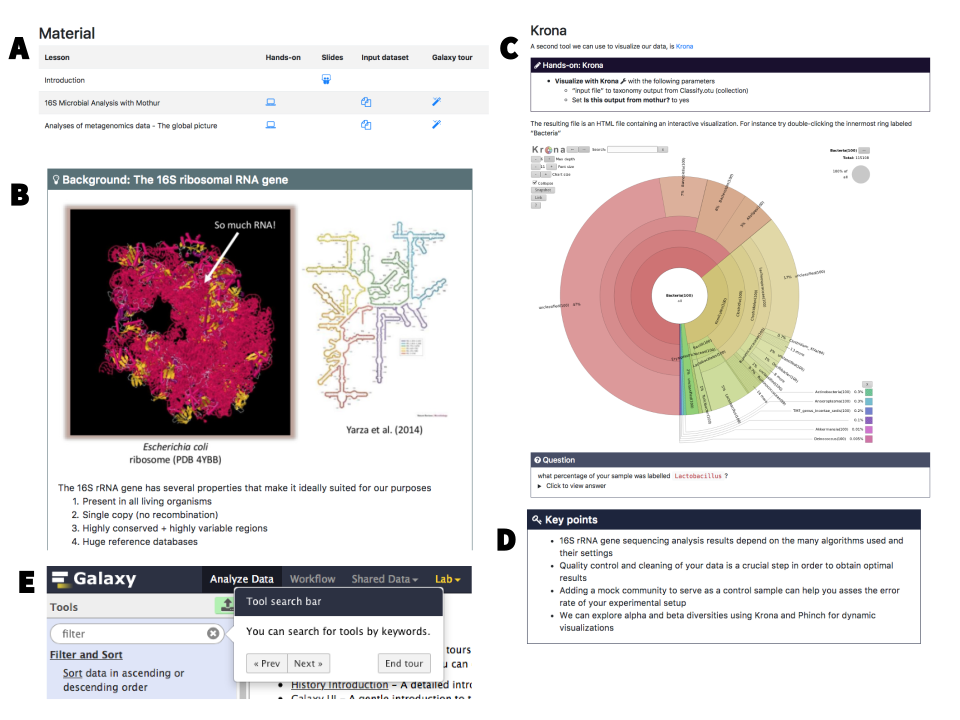
\includegraphics[width=\textwidth]{chapters/images/training-figure-metagenomics.png}
    \caption{ Key elements of an interactive tutorial. \textbf{A.} A list of tutorials dedicated to Metagenomics. There is a set of introductory slides and two hands-on tutorials. \textbf{B.} A fragment of introductory material within a tutorial. \textbf{C.} A “hands-on” element with upper box contains instructions for running a tool inside Galaxy and shown example output of Krona tool. The question box at the bottom contains togglable answer field. \textbf{D.} Summary of key points for this tutorial displayed on the bottom of the tutorial. \textbf{E.} Fragment of Galaxy interface showing interactive tour balloon.  }
    \label{fig:metagenomics}
\end{figure}


\subsection*{Infrastructure to facilitate community-led content development}

\begin{figure}
    \centering
    \includegraphics[width=\textwidth]{chapters/images/training-figure-development.png}
    \caption{Structure and development of content in GitHub (http://github.com/galaxyproject/training-material). The material is organized in different topics, each topic in a dedicated directory. Inside each topic’s directory, the structure is the same: a metadata file, a directory with the topic introduction slide decks, a directory with the tutorials and a directory with the Dockerfile describing the details to build a container for the topic that would contain a dedicated Galaxy instance with all tools relevant for the tutorials. Inside the topic directory, each tutorial related to the topic has its own subdirectory with several files: a tutorial file written in Markdown with hands-on, an optional slides file to support the tutorial, a directory with Galaxy Interactive Tours to reproduce the tutorial, a directory with workflows extracted from the tutorial, a file with the links to the input data needed for the tutorial and a file with the description of needed tools to run the tutorial. The process of development of new content is shown at the bottom of the figure.}
    \label{fig:development}
\end{figure}

To build a comprehensive collection of training materials covering the spectrum of topics in the life sciences, we must leverage community expertise, as no single group can possibly “know it all”. To achieve this goal, we built an infrastructure that makes tutorial creation a convenient, hassle-free process and enables transparent peer-review and curation to guarantee high-quality and current content. In implementing these requirements, we took inspiration from the Software and Data Carpentry \cite{wilson2014software} projects (SDC). In SDC, materials are openly reviewed and iteratively developed on GitHub (\url{https://github.com/}) to capture the breadth of community expertise. SDC delivers training via online tutorials with hands-on sections, which offer better training support than videos because trainees who are actively participating learn more \cite{dollar2007enhancing}.
This format is also adapted to face-to-face courses and self-training, as the content is openly accessible online. The content of these web pages is easy to edit, thus reducing the contribution barrier. The tutorials are developed in Markdown, a plain text markup language, which is automatically transformed into web-browser accessible pages. Using these strategies, we created a GitHub repository (\url{https://github.com/galaxyproject/training-material}) to collect, manage, and distribute training materials.
The architecture of this infrastructure is shown in Fig. \ref{fig:development} (center), with the process for developing a tutorial illustrated at the bottom of the figure. To create a new tutorial, the main repository is forked (duplicated into a user-controlled space) within GitHub by an individual developing the tutorial. The developer then proceeds to write the content using Markdown as explained in our guide at \url{https://training.galaxyproject.org/topics/training} (itself consisting of several tutorials). The guide contains detailed information on technical and stylistic aspects of tutorial development.
After settling on a final version of the tutorial (circles 1 through 10, the bottom of Fig. \ref{fig:development}), a pull request is created against the original repository. When a new pull request is issued, this is an indication that a new tutorial is ready to be reviewed by the editorial team. The team then makes suggestions on the new contents, these suggestions are discussed, and the content is edited accordingly. A decision is then made whether to accept the pull request. At the same time the pull request is first created, the newly added content is automatically tested for HTML generation and all links and images are verified. When the pull request is accepted, the new tutorial becomes a part of the official training material portfolio, and the entire site is regenerated.

This infrastructure has been developed in accordance with the FAIR (Findable, Accessible, Interoperable, Reusable) principles \cite{wilkinson2016fair}. Each tutorial, slide deck, and topic is complemented by numerous metadata described in a standard, accessible, interoperable format (YAML; \url{http://yaml.org/}). The metadata is used to automatically populate the TeSS training portal at the European life-sciences Infrastructure for biological Information (ELIXIR; \url{https://tess.elixir-europe.org}), ensuring global reach \cite{tess2016}. Each topic, tutorial, and slide deck has as metadata a reference to a topic in the EDAM ontology \cite{ison2013edam}, a comprehensive catalog of well-established, familiar concepts that are prevalent within bioinformatics and computational biology. These references can be used to represent relationships among the materials and make them more findable and searchable.

\begin{figure}
    \centering
    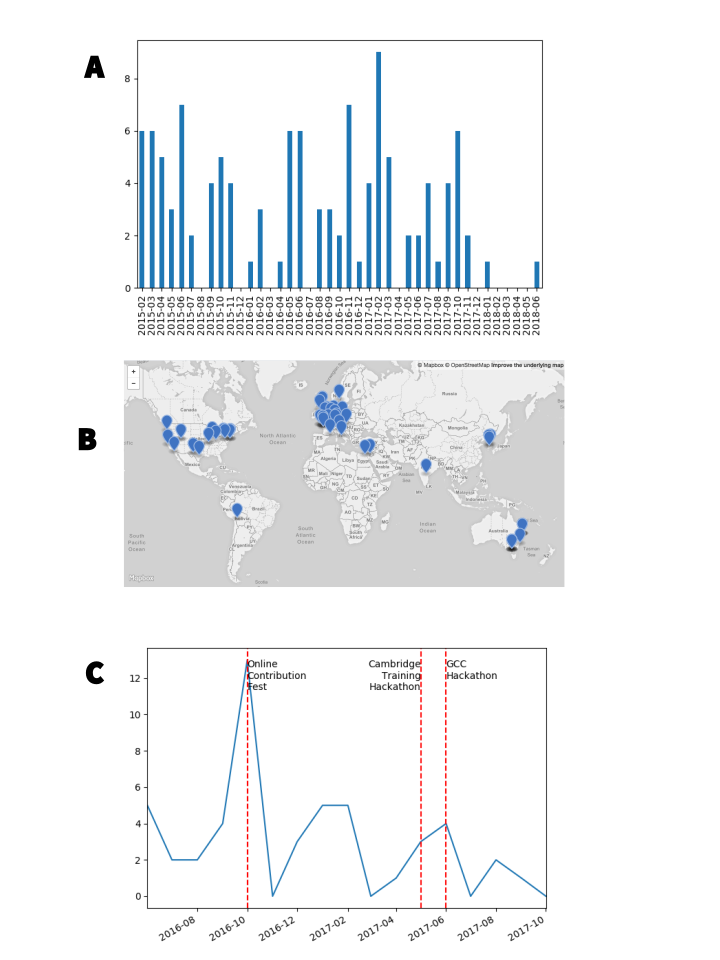
\includegraphics[width=400pt]{chapters/images/training-figure-stats.png}
    \caption{History of training activities. Number (A) and location (B) of registered training events organized by the Galaxy Training Network since 2015. C. Number of tutorial contributors per month.}
    \label{fig:stats}
\end{figure}

Using the framework described above, we relaunched the Galaxy Training Network (GTN; \url{https://galaxyproject.org/teach/gtn}). This growing network currently consists of 33 scientific groups (\url{https://galaxyproject.org/teach/trainers}) invested in Galaxy-based training. The GTN regularly organizes training events worldwide (Fig. \ref{fig:stats}) and offers best practices for developing Galaxy-based training material, advice on compute platform choice to use for training, and a catalog of existing training resources for Galaxy (Table \ref{table:tutorialtable}).

\subsection*{Ensuring accessibility of tutorials}
Most training materials hosted within the GTN resource are intended to be used side-by-side with the Galaxy framework. However, the public Galaxy instances (e.g. \url{https://usegalaxy.org} or \url{https://galaxy.uni-freiburg.de}) are occasionally subject to unpredictable load, may be inaccessible due to network problems in remote parts of the world or may not have all the tools necessary for completing the tutorials. To account for these situations, we have developed a Docker-based framework for creating portable, on-demand Galaxy instances specifically targeted for a given tutorial. Docker (\url{https://www.docker.com}) is a container platform which provides lightweight virtualization by executing "images" (files that include everything needed to run a piece of software) isolated from the host computer environment. An individual creating a new tutorial lists all tools that are required to complete it in a dedicated configuration file (tools file, Fig. \ref{fig:development}). For example, a metagenomics tutorial uses the mothur \cite{schloss2009introducing} set of tools as well as visualization applications such as Krona \cite{ondov2015krona}. The corresponding Galaxy tools are listed in a configuration file that is a part of the metagenomics tutorial. This file is used to install these Galaxy tools and their dependencies into a base Galaxy Docker image (containing essential Galaxy functionality and a core set of tools) to create a dedicated “on-demand” Galaxy instance which can then be used on any trainer’s or trainee’s computer. The Docker image also contains input data, tours, workflows.

\section*{A vision for the future}
Life sciences are on a trajectory towards becoming an entirely data-driven scientific domain. A growing understanding that biomedical curricula must be modernized to reflect these changes is gaining attention \cite{10.7554/eLife.32715}. Our project represents one of the first fully open, “grass-roots” attempts at unifying and standardizing heterogeneous training resources around the Galaxy platform. While it may not be appropriate to all, our multi-year experience with teaching workshops at various skill-levels can be summarized as the following set of recommendations, which we use as guiding principles. These recommendations may also be useful for the development of alternative frameworks as well as for curriculum planning:

\begin{enumerate}
\item \textbf{Require quantitative training.} No one expects biomedical researchers to rival their colleagues in departments of mathematics or statistics. However, background level statistical reasoning must be included in all training materials and general statistical courses must become a part of undergraduate and graduate education. This would have an enormous positive impact on the quality of biomedical research because researchers with basic understanding of quantitative concepts will not, for example, perform an RNAseq experiment without a sufficient number of replicates.
\item \textbf{Demystify computational methodologies.} Fundamental principles, limitations, and assumptions of molecular experimental techniques are typically well understood by biomedical researchers even when proprietary reagent kits are used. This is not the case with software tools, which are often treated as black boxes. We argue that fundamental principles of bioinformatic techniques (e.g., read mapping, read assembly) must be understood by experimentalists as this will also lead to an increase in overall quality of research output.
\item \textbf{Advocate the fundamental virtues of open and transparent research.} Open and transparent data analysis (e.g., through the use of open-source software) promotes replication and validation of results by independent investigators. It also speeds up research progress by facilitating reuse and repurposing of published analyses to different datasets or even to other disciplines. We advocate openness as a basic principle for computational analysis of biomedical data.
\end{enumerate}

The infrastructure presented here has been developed to support training using Galaxy, a powerful tool for teaching bioinformatics concepts and analysis. But such a model is not only limited to Galaxy. It could be applied to bioinformatics training more generally (and to other disciplines as well) to support learners and instructors in this ever-changing landscape that is the life sciences.


\section*{Acknowledgments}
The authors are grateful to the Freiburg Galaxy and Core Galaxy teams, as without these resources this work would not be possible. Adoption of Galaxy Tours has been accelerated with the introduction of Galaxy Tour Builder (\url{https://zenodo.org/record/830481}) by William Durand (\url{https://tailordev.fr}). This project was supported by Collaborative Research Centre 992 Medical Epigenetics (DFG grant SFB 992/1 2012), German Federal Ministry of Education and Research (BMBF grant 031 A538A RBC (de.NBI)), NIH Grants U41 HG006620 and R01 AI134384-01, as well as NSF Grant 1661497.
References


\bibliographystyle{plain}
\bibliography{references}

\begin{savequote}[75mm]
This is some random quote to start off the chapter.
\qauthor{Firstname lastname}
\end{savequote}

\chapter{iFUSE \& VCaP Chromothripsis}


\includepdf[pages=1-2]{chapters/myarticles/iFUSE.pdf}

\includepdf[pages=1-5]{chapters/myarticles/VCaP.pdf}


\bibliographystyle{plain}
\bibliography{references}

\begin{savequote}[75mm]
Nulla facilisi. In vel sem. Morbi id urna in diam dignissim feugiat. Proin molestie tortor eu velit. Aliquam erat volutpat. Nullam ultrices, diam tempus vulputate egestas, eros pede varius leo.
\qauthor{Quoteauthor Lastname}
\end{savequote}

\chapter{Somatic Variant Detection}
\label{chapter:virtualnormal}
\setcounter{figure}{-1}
\setcounter{table}{-1}
\setcounter{section}{-1}

We integrated the Complete Genomics toolsuite into Galaxy and used it to analyse tumour samples without a matching normal.


\cleartoleftpage
%\begin{center}
%\vspace{2cm}
%\begin{minipage}{5in}
%\cleartoleftpage
\tikz[remember picture,overlay]
\node[opacity=0.8,inner sep=0pt] at (current page.center){\includegraphics[width=\paperwidth,height=\paperheight]{frontmatter/images/border-1.png}};
\thispagestyle{empty} %remove page number?
\begin{center}
\vspace*{-0.5cm}
{\Large Scaling the Researcher \normalsize
\small

\vspace*{0.3cm}
\includegraphics[scale=0.1]{chapters/images/discussion/dana.png}
% image from: https://www.kissclipart.com/data-analyst-png-clipart-data-science-data-analysi-fk1hr4/download-clipart.html
\vspace*{0.3cm}

Meet Dana.
Dana is a biologist who studies DNA\@.
Dana sends her samples out to be sequenced, and gets back hard drives full of files.
However, she doesn't really know what to do with these files.
She tries opening a VCF file in Excel, but it complains that there are too many lines and immediately closes.
She double clicks on a FASTQ file, and her computer freezes while trying to open the file in Notepad.

Luckily her group has a bioinformatician, Bindi, surely they can just do the analysis for her!
Bindi tells her she is very busy right now doing analysis for the group, and can look at her files in a few months, hopefully.
Dana just wants to analyse her data and publish her paper! She doesn't want to wait months, so she tries analyzing her data herself.
She finds some tools in the literature but when she tries to install them, she sees they cannot be run on Windows, what now?
She gets access to a Linux compute server, but the tool she wants does not install properly.
There are no good instructions on how to fix the problem.
She tries a different tool, which does install, but when she runs it on her own data, she gets some cryptic error messages.
\emph{"Only bioinformaticians could make sense of all this!"}, she sighs.

Then somebody tells her about Galaxy.
It has the tools she wants, and she doesn't even have to install anything, all she has to do is click buttons in her browser!
And it's free!
Galaxy is not easy, but there are a lot of useful training materials available.
She teaches herself how to use Galaxy, and how to analyze her data. She reads papers and reproduces their methods in Galaxy.
She gets stuck, but asks for help from the community.
She goes to workshops to learn more.
It was a lot of work, but she gets some promising results! She has another batch of samples on the way. She creates a workflow to speed up the analysis next time.

Her coworkers also want to analyze their data.
Bindi the bioinformatician is still very busy, and the queue is long, so they ask Dana for help.
Dana shares her Galaxy workflow with them.
She gets a lot of emails with questions from her coworkers, so she decides to create her own Galaxy tutorial about the workflow.
Dana teaches a workhops, training her colleagues on how to use Galaxy and her workflow.

Dana publishes her paper. Dana is happy.
With researchers in the group now running their own day-to-day analyses, Bindi the bioinformaticians has more time.
She can use this time to add new tools to Galaxy, create workflows for the group, and develop training materials for her coworkers to use. Bindi is happy too.
\normalsize
}
\end{center}
%\end{minipage}
%\end{center}

\cleartorightpage

\begin{savequote}[75mm]
``Humans are allergic to change. They love to say, `We've always done it this way'. I try to fight that. That's why I have a clock on my wall that runs counter-clockwise.''
\qauthor{Grace Hopper}
\end{savequote}

\chapter{Discussion}\label{discussion}
\setcounter{figure}{-1}
\setcounter{table}{-1}
\setcounter{section}{-1}
\setcounter{NAT@ctr}{-1}

\begin{figure}[t!]
\includegraphics[height=15em]{frontmatter/images/chapter-header-discussion-tools.png}
\end{figure}
\setcounter{figure}{-1}
\setcounter{table}{-1}
\setcounter{section}{-1}


\emph{"Bioinformatics has become too central to biology to be left to specialist bioinformaticians"} notes Lincoln Stein in 2008 \cite{stein2008bioinformatics}.
And indeed, bioinformatics now plays a vital role in almost every biological and biomedical research project.
Data is being generated at an exponential rate, but bioinformaticians are not,  and it is not scalable to leave the analysis of all this data to specialist bioinformaticians.
Much of the discussion around the challenge of scaling to meet the needs of this data deluge tends to focus on the need for scaling up compute resources and data storage.
And while these are both very important factors, the much greater challenge lies in scaling not just the analysis itself, but the interpretation of all this data.
And nobody is better suited for this task than the research scientists themselves. So the question now becomes: \emph{How can we scale the researcher?}

The answer to this question lies in empowering researchers to run their own data analyses again.
The way we achieve this is by shining a light in the black box of bioinformatics.
This entails making bioinformatics tools and pipelines accessible and easy to use for domain scientists.
It requires training of researchers not just in how to use these tools, but also basic knowledge about the computational methodologies, and any biases these may introduce that can impact the interpretation of results.

This is not to say there is no role for bioinformaticians.
It takes a lot of work to make analysis accessible, but by enabling research scientists to handle their own day-to-day analyses, we free up bioinformaticians to focus on the development of new and better tools, for configuring new workflows, improving reproducibility, and developing and delivering training.

Therefore, in this thesis we set out to develop a user-friendly, open, and FAIR bioinformatics framework for NGS analysis, so that we can create a community of researchers who are computationally informed.
We then applied this paradigm to a series of research projects to illustrate its utility.


%Since the completion of the human reference genome in 2003, the field of molecular biology has been transformed almost beyond recognition, and along with it, the field of bioinformatics has evolved from a niche discipline to an integral part of every biomolecular research question. Where decades ago most genomic data analyses could largely be performed by hand, nowadays they often require a supercomputer. Programming knowledge is required to run such analyses, but biomedical scientists are not typically trained in these skills, and have thus become reliant on bio\-infor\-ma\-ticians to carry out this work for them. Similarly, bioinformaticians often lack the increasingly complex biological knowledge required to fully interpret the results~\cite{preeyanon2014reproducible}. Biologist and bioinformatician must therefore work together closely, and each should be trained in the other discipline in order gain awareness of factors that might influence analysis or result interpretation.

%Furthermore, data is being generated at an exponential rate (while bioinformaticians are not), and one way to address this gap is to empower researchers and clinicians to run their own day-to-day analyses without the need to consult a bioinformatician at every step. A way towards delivering this is through the creation of accessible analysis tools and platforms and sufficient training resources.


\section{Accessible Bioinformatics}

The main challenge in our aim of scaling the researcher, is making bioinformatics accessible for non-bioinformaticians. This includes not only making analyses easy to use, but also easier to understand and interpret.
In our approach we used the Galaxy platform to provide a user-friendly interface to bioinformatics analyses. Galaxy does all the heavy lifting of handling installation of the tools and all their dependencies, of optimally scheduling jobs across the compute resources, tracking provenance of analyses, enabling sharing, and much more. This leaves the researcher free to focus the interpretation of their results.
The second main component of our approach to making bioinformatics more accessible consists of providing extensive bioinformatics training. To this end, we founded the Galaxy training materials project, a collaborative framework for development and maintenance of training materials using the Galaxy framework.


\subsection{Galaxy as a user-friendly workflow platform}

The Galaxy project~\cite{giardine2005galaxy,blankenberg2010galaxy,afgan2016galaxy} enables researchers to run complex data analysis without programming expertise, directly from their web browser. While there are several workflow management systems \cite{clcbio,taverna,onlinehpc,anduril,molgenis}, some of these solutions are commercial and may not be affordable to many labs, others require local installation, prohibiting scaling to accomodate large datasets. Furthermore, many solutions are not open source, meaning only the core development team can provide updates to the platform, limiting flexibility of the platform to its end users.

In contrast, Galaxy is completely free and open-source, and perhaps its most attractive asset is the very large and active user and developer community behind it. Galaxy encourages feedback and code contributions from its users to improve the platform, and evolve along with the ever-changing landscape that is bioinformatics. This paradigm means that anybody is able to add features to Galaxy or provide bug fixes, and can share those enhancements back to the main code base, thereby enabling a much faster and more flexible development cycle.

Galaxy continues to increase in popularity, illustrated by the exponential growth of both the number of available tools (over 8000) \cite{galaxytoolshed}, and the number of publication citing Galaxy (almost 10,000) \cite{url-zotero-galaxy}.
\hyperref[chapter:galaxy]{\textbf{Chapter~\ref{chapter:galaxy}}} outlines the ongoing development in the Galaxy framework. One of the major improvements was in the handling of big data. Galaxy addresses this issue by introducing the concept of data collections. This allows users to easily scale their analyses up from single datasets to hundreds of thousands of samples at once, using the exact same procedures they have grown accustomed to.
However, the greater challenge of big datasets is not just the processing of the files, but rather managing all this data in an effective way.
To support the organisation of these large number of samples in Galaxy, the rule-based uploader was created, a novel feature which essentially allows sample sheets to be uploaded alongside the raw data files, and the metadata stored within them to be coupled to the datasets in Galaxy.

While the Galaxy project certainly greatly improves accessibility of bioinformatics analyses, there are still a number of areas of improvement remaining.
For example, with sequencing now widespread and affordable, it has become feasible to use NGS directly in the clinic to inform patient care.
However, until now Galaxy has focused mainly on researchers, and in order to make Galaxy more appealing for clinicians, the framework could benefit from a number of additional features.
Firstly, a \emph{locked-down}, workflow-centric user interface is required; in contrast with research applications where Galaxy's great flexibility is an asset, for clinical applications this flexibility can be a hindrance, as it goes hand in hand with added complexity.
Unlike researchers, clinicians do not typically need to play around with their datasets and try different tools; their analysis options should be limited to a small set of predefined and thoroughly validated analysis pipelines.
While Galaxy does not (yet) offer such an alternate user view, it does offer API access to its framework, enabling custom front-ends to be developed on top of the Galaxy back-end.
The need for such a simplified user interface to Galaxy is exemplified by the number of projects that have developed such a customized front-end to the Galaxy interface \cite{klingstrom2017galaksio,matthews2018integrated,lemoine2019ngphylogeny,SEEK2015}, including several in-house projects at the ErasmusMC\@.
For example, the IRIDA (Integrated Rapid Infectious Disease Analysis) project \cite{matthews2018integrated} is an open-source platform for public health genomics, which is currently in use by the Canadian public health agency to track infectious disease outbreaks.
It uses Galaxy as its analysis platform, but provides a custom user interface tailored specifically to the needs of its users. This approach also enabled the project to integrate Galaxy directly with a third-party data management system where users can easily mange their projects and data.
While Galaxy does not aim to be a data management system, in this big data era it has become increasingly imperative to offer good data management solutions to researchers. Therefore, integrations of Galaxy with third-party data management systems in the future could profoundly increase usability of the platform even further.

We used Galaxy as the main data analysis platform in each of the 3 research projects described in this thesis, including one clinical analysis platform (MYcrobiota). For several of these publications, we were able to submit our Galaxy history and workflows directly to the journal as a full end-to-end demonstration of our analysis pipeline, which could then be used to reproduce our results by reviewers and readers.


\subsection{Visualisation and Reporting}
Visualisation is an essential component to aid in interpretation of big and multidimensional datasets. Tools such as Circos \cite{circos} allow for the visualisation of multiple large and complex datasets in a single circular plot. Circos is highly customizable, but this high degree of flexibility comes paired with a high degree of complexity and a steep learning curve. To improve the user-friendliness of this tool and improve its interoperability with upstream tools, we developed Galactic Circos (Chapter~\ref{chapter:general}), integrating Circos into Galaxy, and providing a set of preprocessing tools to support integration with a wide range of input file formats.

The Circos visualisation tool was especially useful in discovery of chromothripsis of the VCaP sample (Chapter~\ref{chapter:vcap}).
Here the highly rearranged nature of chromosome 5q was instantly obvious in one glance at the circular plot, in a way that simply inspecting the textual files listing the SVs could not convey.

Effective visualisation of large data is crucial for the interpretation of analysis results, and in a broader sense, so is the reporting of results in a single, easily-digestible overview or report. Analysis pipelines often result in a large set of different output files, and displaying these results effectively to the end user tasked with interpretation of the results is a challenge in its own right.
Galaxy in its current form lacks an appealing system of results summation and reporting. While Galaxy sports a plugin system for visualisation of individual datasets, a generic reporting tool for displaying a set of workflow outputs together does not exist. To this end, we developed iReport (Chapter~\ref{chapter:general}); a fully customizable Galaxy tool for the generation HTML reports capable of displaying any number of workflow outputs.\

iReport is intended to be used as the final step of a workflow, and is generic enough that it makes no assumptions about the underlying analysis or scientific domain.\ iReport supports  the ability to add links to datasets and external resources, create searchable and sortable tables, embed images and custom text, and to structure content into different pages.
By adding such a summarizing report at the end of an analysis pipeline, clinicians and other end users are able to run workflows and view results with minimal instruction or knowledge of the Galaxy interface.
We used iReport as the reporting tool for the MYcrobiota clinical analysis platform (Chapter~\ref{chapter:mycrobiota}), based on the requirements of the clinicians at the Streeklab Haarlem.

Since the development of the iReport tool, the need for a reporting system more tightly integrated with the Galaxy framework itself was recognized by the Galaxy core team, and they have since started to integrate similar functionality into the Galaxy code base. While this reporting system is relatively new and does not yet support the full functionality of iReport, we are hopeful that continued development here will improve Galaxy's reporting mechanisms.

\subsection{Training}
Training is an essential component in the dissemination of accessible bioinformatics tools and workflows. The Galaxy platform is especially well-suited for the delivery of bioinformatics training because it provides a layer of abstraction that allows trainees to focus on the bioinformatics \emph{concepts} rather than the implementation details of the tools. Without this separation, trainees would have to simultaneously learn about the UNIX commandline or programming environment, on top of the bioinformatics topics at hand. This would increase the cognitive load and hamper the learning process~\cite{paas2003cognitive}. Given this observation of Galaxy's suitability for use in training, the Galaxy Training Network (GTN)~\cite{url-gtn} was formed; a loosely-defined open group of instructors around the world who use Galaxy for training purposes. Initially there was little coordination between the different instructors in terms of materials used, and thus a lot of duplication of effort. There was a clear need for centralisation of training materials and knowledge sharing within the trainer community. Chapter~\ref{chapter:training} describes the community-driven web-based framework for the delivery of bioinformatics training using the Galaxy platform that we developed in response to this need.
Our aim was to create a fully open and transparent framework that is accessible and easy to use for both trainees and trainers. The materials are centered around \emph{research stories}; usually the recreation of results described in published papers. This gives trainees the confidence that the tools and pipelines are practically useful and of publication-level quality, as well providing them with the opportunity to dive deeper into the science and informatics behind the training. Since the creation of this training platform, a number of scientific publications have included Galaxy training materials as a form of documentation and illustration of the presented analysis pipelines~\cite{gruning2017rna,blank2018disseminating,batut2017asaim,hiltemann2018galaxy}.

One of the main challenges in designing this framework was to allow easy contributions from instructors, without the need for any web development knowledge. To this end, we used Jekyll templating~\cite{url-jekyll}, which allows tutorials to be written in the simple and accessible markup language called Markdown~\cite{url-markdown} which can be rendered as HTML\@. Analogous to how Galaxy allows scientists to run analyses while being abstracted away from the implementation layer of the tools, this approach allows instructors to create web pages for their tutorials without being concerned with the syntax and intricacies of the web application layer.

A further challenge was to enable the materials to be usable both by instructors during workshops, and by individuals learning on their own. This is accomplished by including all materials instructors might provide during a workshop in the GTN training materials framework. This includes introduction slides as well as hand-on materials, input datasets and workflows, further reading suggestions, and an automatically updated list of available Galaxy servers which meet the requirements to run a given tutorial. Furthermore, learning assessments are provided in the form of question boxes, answers to which are included within the materials (in an initially hidden state) for trainees to verify their understanding of the materials. If further assistance is required, links to support channels such as a help forum and chat rooms are provided.

The community-driven nature of the training framework is essential for the long-term survival of the project; it allows for the distribution of the maintenance burden and takes advantage of the combined expertise present in the community. All development happens on GitHub~\cite{url-github}, where anybody may suggest additions or changes, and any such proposed changes are thoroughly tested using the Travis continuous integration system~\cite{travis-ci} to ensure functionality and adherence to guidelines. The proposed changes are subsequently reviewed by one or more of the dedicated topic maintainers, or other volunteers from the community. Once approved, the code is merged into the main code base, and the new website is automatically built and deployed using Travis and GitHub. In order to assess the quality of the tutorials and identify areas of improvement, feedback from both trainees and instructors is indispensable. To this end, we integrated evaluation forms at the end of each tutorial, and hold regular community meetings with tutorial authors and trainers.

As Galaxy evolves, so will the associated tutorials; where Galaxy is expanding beyond bioinformatics and is now also being used in fields such as natural language processing and computational chemistry, so have we noticed a steady expansion of topics and tutorials contributed by the community. In the year following the publication of Chapter~\ref{chapter:training} , we saw 6 new topics added, 66 new tutorials, and the number of contributors grew from 64 to 137.

While the focus of development in this project initially lay with improving the experience for end-users of the tutorials, our focus is now shifting to increasing support for tutorial contributors and instructors intending to use our materials. The main challenge in the coming years will be the community management; creating and sustaining a close-knit community of Galaxy users and instructors so that the project can survive even when its original developers have moved on.

While this project focuses on the training of research scientists to effectively use bioinformatics analyses, the reverse is also important; much like bioinformatics may feel like a \emph{black box} to researchers and clinicians, so can the wetlab seem like a black box to many bioinformaticians.
Bioinformaticians typically work on multiple projects at the same time, often covering a variety of different scientific domains, and therefore can not acquire the same level of knowledge about the underlying biology as the domain specialists.
However, similar to how researchers and clinicians will benefit from a basic knowledge of computational concepts to aid the interpretation of analysis results, so do bioinformaticians need a minimum knowledge of the scientific domains in order to optimally develop their tools and workflows.
The tutorials in the GTN framework are generally aimed at novices and as a result can also be used by bioinformaticians to acquire knowledge of the basic concept involved in different scientific domains.
However, I would love to see a project conceptually similar to the GTN training materials framework, but explicitly aimed at training bioinformaticians in the relevant biological concepts.


\section{Use Cases}

The concepts and tools described in the previous sections were applied to two separate use cases. Chapters~\ref{chapter:fusiongenes} and~\ref{chapter:virtualnormal} describe the creation of analysis tools and pipelines for variant analysis in prostate cancer research. In Chapter~\ref{chapter:microbiota}, Galaxy-based analysis pipelines were developed and tested for the application of NGS-based microbiota profiling for clinical diagnostics.


\subsection{Cancer Analysis: Structural Variant Analysis}
\subsubsection{The Bio}

Cancer is a disease of the genome, where DNA mutations accumulate over time and wreak havoc on the cell. Our best hope in defeating this disease lies in the full characterization of the cancer cell, not only in terms of their observed mutational signatures, but also the mechanisms behind these mutational landscapes.

While small-scale mutations that affect the protein-coding regions of the genome have been widely studied, the impact of non-coding mutations and large-scale structural variants (SVs) in cancer remain largely undefined~\cite{cuykendall2017non,khurana2016role}. Now that whole-genome sequencing has become more available and affordable, a comprehensive characterization of SVs has become possible.

Large-scale genomic rearrangements have the potential to lead to the generation of hybrid genes known as fusion genes.
Accurate detection of such fusion genes may aid in the diagnosis or treatment of cancer~\cite{nowell1960chromosome,nowell1961chromosome,druker2001activity,druker2001efficacy}.
Prostate cancer was among the first solid tumours demonstrated to harbour frequent large-scale genomic rearrangements, demonstrated by the discovery of the \emph{TMPRSS2-ERG} fusion gene, which was found to be present in approximately 50\% of all prostate cancers \cite{tomlins2005recurrent}.
Subsequent studies have shown that point-mutations occur relatively infrequently in prostate cancer as compared to structural variations and extensive copy-number variation, suggesting that it is these large-scale genomic rearrangements that are the primary driver of prostate cancer progression \cite{taylor2010integrative,rubin2011common}.

Understanding the mechanisms behind the acquisition of these structural variations will provide valuable insights into tumor progression.
While historically the acquisition of mutations in tumour cells has been thought of as a gradual and incremental process, subsequent insights have uncovered several mutational processes capable of generating large numbers of mutations in a single event \cite{cortes2020comprehensive,willis2015}.
Kataegis (from the greek word for thunderstorm) represents a \emph{mutation storm} of localised hypermutations, and has been observed in multiple cancer types \cite{nik2012mutational,davis2014somatic}.
Chromothripsis is a shattering of the genome --often an entire chromosome or chromosome arm-- followed by a highly erroneous repair step \cite{stephens2011massive,maher2012chromothripsis}.
Chromoplexy (from the Greek \emph{pleko}, which means to weave) is a phenomenon where large chains of rearrangements affecting multiple chromosomes occur \cite{shen2013chromoplexy}. All these mechanisms challenge the classical view of cancer progression as a gradual and step-wise process.

In Chapter~\ref{chapter:vcap} we showed that chromothripsis also occurs in prostate cancer, by describing the identification of chromothripsis in the 5q arm of the VCaP cell line. A very large number of SVs were detected, and copy number varied primarily between two copy number states states, with only sporadic occurrences of a third state. This alternation between a small number of copy number states suggest the rearrangements were precipitated by a single catastrophic event.
Other studies have also observed chromothripsis in other prostate cancer samples \cite{wu2012poly,Baca2013}.

Such a high degree of genomic rearrangement has the potential of contributing to cancer progression e.g.\ through activation of oncogenes, or inactivation of tumor suppressor genes.
To investigate this further, we evaluated the 573 rearrangements involving the impacted region of chromosome 5 for their potential to lead to the formation of fusion genes, using the iFUSE application presented in Chapter~\ref{chapter:ifuse}.
Out of this large number of rearrangements, a relatively small number (18) were found to occur between two different genes at a consistent orientation, with only 2 predicted to be in-frame by the iFUSE application.
Out of the 18 fusion candidates identified, 16 were confirmed on the DNA level using custom PCR\@.
Only 5 of these were also measured on the mRNA level, suggesting instability of the fusion transcripts or down-regulation of the expression of these fusion genes.
Therefore, our results suggests that chromothripsis does not preferentially impact coding regions and that there is no positive selection for in-frame fusion transcripts.

Overall, our research has shown that any studies involving this commonly used prostate cancer cell line should take the presence of chromothripsis on chromosome 5q into account.
Furthermore, this study highlights the potential utility of this cell line as a model for research on chromothripsis.

Chromothripsis has been observed in many other cancer types as well, with the frequency of occurrence varying greatly across tumour types \cite{cortes2020comprehensive,voronina2020landscape,Koltsova2019,kloosterman2014prevalence}.
A study examining 2,658 WGS patient samples obtained from the ICGC and TCGA projects found pervasive chromothripsis across all 38 cancer types examined. The prevalace varied significantly by tumour type, with liposarcomas (100\%) and osteosarcomas (77\%) on the high end, and thyroid adenocarcinomas (3.3\%) and chronic lymphocytic leukemia (1.2\%) on the lower end of the spectrum \cite{cortes2020comprehensive}.
It must be noted that due to the variability in detection methods and in the precise definition and criteria of chromothripsis used in different studies, the exact numbers vary significantly in the literature, though the variability across different tumour types is consistently observed.
Chromothripsis has been shown to be associated with poorer outcome \cite{fontana2018chromothripsis,Hirsch2012,magrangeas2011chromothripsis,molenaar} and accurate detection of the presence of chromothripsis could therefore provide clinically relevant prognostic value.


%Prostate cancer is one of the most commonly diagnosed cancer types in men, and while many patients present with an indolent form of the disease, others develop a highly aggressive tumour type, and overall, prostate cancer is among the top 10 leading causes of cancer-related deaths in men~\cite{jemal2010global}.
%Cancer is a disease of the genome, where accumulation of mutations over time drive the progression of the illness. Genome sequencing approaches can be used to extensively explore these genomic alterations in cancer, including small variants and larger structural variants (SVs), within or ouside genes.

%The advent of whole-genome sequencing techniques has enable the characterization of SVs and other mutations not detectable by exome-based approaches.
%Fusion genes may arise when structural variants (SVs) occur within two different genes, causing the creation of hybrid genes with the potential to produce hybrid proteins that may disrupt vital cell functions.
%For example, the presence of the \emph{TMPRSS2-ERG} gene fusion is observed in approximately 50\% of prostate cancer patients and many other less frequent fusions have also been identified~\cite{tomlins2005recurrent}. Detection of fusion genes may aid in the diagnosis or treatment of cancer~\cite{nowell1960chromosome,nowell1961chromosome,druker2001activity,druker2001efficacy}.

%Chromothripsis is a phenomenon observed primarily in cancer cells, that involves the shattering and subsequent imprecise repair of one or more chromosomes in a single catastrophic event. Chromothripsis is characterized by the observation of 1) large numbers of chromosomal rearrangements on a localized parts of the genome, 2) alternations between a small number of different copy number states, and 3) alternation between regions displaying a loss of heterozygosity (LOH) and those with preserved heterozygosity~\cite{maher2012chromothripsis}.



%chromoplexy (chains) in PCa - \cite{Baca2013}


\subsubsection{The Informatics}
Whole-genome sequence experiments typically generate very large output files, and interpretation is greatly aided by visualisation and annotation with external data resources.  Furthermore, in the case of structural variant analysis, the output file formats lack consistency across tools and sequencing platforms. To this end, the iFUSE application was developed; it supports multiple input formats, and creates a visual representation of fusion gene candidates and computes various metrics such as predictions of fusion protein product.

While iFUSE provides valuable aid in interpretation on a per-event basis through its visualisation and annotation, it is less suitable for obtaining a genome-wide overview of structural rearrangements. Large-scale rearrangements such as chromothripsis for instance are easy to miss when examining the raw textual output files or the iFUSE visualisations. In order to evaluate the presence of chromothripsis, a more high-level view of the genome is needed, and to that end, whole-genome visualisations were created using Circos~\cite{circos} for rearrangements, and GNUplot~\cite{url-gnuplot} for the copy number and heterozygosity plots. This approach enabled the instant identification of chromothripsis present in the VCaP sample, which could then be followed up by closer examination of individual rearrangements involving the chromosome 5q using iFUSE.

Both the iFUSE application, the Circos Galaxy wrappers, and the other tools and visualisations created in this chapter are open-source and publicly available on an example server, and are accompanied by extensive documentation to enable re-use by institutes that may have legal restrictions about the use of clinical samples on public servers.

If we want to go beyond the mere detection of chromothripsis to the prediction of the effects of these catastrophic events on the cell, we will have to fully reconstruct the tumour genome.
While algorithms have been developed for the reconstruction of structurally rearranged genomes \cite{prego,Baca2013}, none of these methods is currently capable of handling the high degree of rearrangement observed in some cancers, let alone those harbouring chromothripsis.
This appears to be a limitation of the power of the data yielded by short-read techniques, rather than a shortcoming of the algorithmic methods.
The recent advances in long-read sequencing techniques will provide valuable improvements for reconstructing cancer genomes impacted by chromothripsis by providing reads spanning multiple breakpoints.
Indeed, this method was employed recently for the successful reconstruction of a genome impacted chromothripsis in a patient with the rare genetic Langer–Giedion syndrome~\cite{lei2020long}.
Similar approaches could be used to reconstruct highly rearranged tumour genomes and have the potential to significantly increase biological insight into the effects of chromothripsis events on the cell.

\subsection{Cancer Analysis: Somatic Mutation Determination}
\subsubsection{The Bio}
One of the main challenges in analysis of oncological samples is the identification of those mutations that potentially function as oncogenic drivers, and the large number of passenger mutations or polymorphisms present in the germline of the patient that are typically deemed to be functionally benign~\cite{lawrence2013mutational}. To this end, a sample of normal tissue from the same individual is often sequenced in conjunction with the tumour sample. This allows the subtraction of germline variants from the set of mutations detected in the cancer sample, in order to narrow down the set of potential driver mutations. However, in practice such an associated normal sample may not always be available, for a variety of reasons. In such cases, an alternative approach is required.

Given the observation that the majority of any individuals germline variants are polymorphic and observed frequently throughout the human population~\cite{10002010map,10002012integrated}, in combination with the exponential increase in publicly available genomic datasets, we explored the feasibility of constructing a so-called \emph{virtual normal}, consisting of a reference set of variants found in the population. Chapter~\ref{chapter:virtualnormal} describes this investigation.

Our approach used a set of over 900 publicly available whole genomes from healthy, ethnically diverse individuals. We combined this with the customary approach of annotating variants for presences in several online databases of polymorphism in the human population. We tested the performance of our method using 4 different tumour samples with associated normal samples, 2 of which had been sequenced on two different platforms (Complete Genomics and Illumina).

Our results show that while highly unique personal variants cannot be 100\% corrected for, a significant number of variants observed in the tumour sample also occur in the virtual normal set of genomes, and thus can be corrected without the need of an associated normal sample from the same individual. As more and more WGS samples are made publicly available, increasingly rare variants may be corrected for in this manner. Furthermore, we demonstrated that the use of a virtual normal provided a significant improvement over relying solely on annotation with online variant databases. This observation seems counter-intuitive given that these databases often contain variants originating from tens of thousands of sequencing experiments; far more genomes than the virtual normal. However, this result can be explained by noting that the virtual normal approach preserves the genomic context of variants (e.g.\ adjacent variants in the same sample), while this contextual information is lost when variants are submitted to variant databases. To understand why this contextual information is so important, one must realize that many mutations can be described in multiple different yet equivalent ways, and the only way to resolve this equivalency is to take the genomic neighbourhood of the variants into account. This enables more advanced comparison algorithms to resolve equivalency of variants where routine position-based exact comparison method fall short.

A combination of all 3 correction methods (matched normal, virtual normal, and variant databases) yields optimal results, but when faced with a choice between a virtual normal or a matched normal, both approaches performed roughly equally well. Without an associated normal, personal germline variants may be erroneously deemed somatic, but conversely, omission of the virtual normal led to a roughly equal number of false-positive somatic variants. This can be explained by a combination of sequencing errors or suboptimal variant calls in the associated normal sample, and the general difficulty present in variant comparison analyses.

Depending on the use case, the decrease in power to detect highly personal germline variants may be offset by the decrease in cost from the absence of the necessity of sequencing a matched normal sample with every tumour sample.

\subsubsection{The Informatics}
The samples in this study were sequenced by Complete Genomics~\cite{drmanac}, a sequencing service which delivers both raw sequencing data and post-processed results. Complete Genomics provide a suite of commandline tools for handling and downstream analysis of their often custom file formats. As a first step towards building the virtual normal analysis pipelines, these existing tools were wrapped into Galaxy. On top of these third party tools, several custom analysis components had to be created, as well as several file format conversion steps to function as a \emph{glue} between steps. The full suite of analysis tools has been made publicly available on GitHub, as well as detailed instructions on where to obtain the virtual normal genome set, and how this may be extended with additional normal samples in the future.


\subsection{Microbiota Profiling for Clinical Diagnostics}
\subsubsection{The Bio}
The MYcrobiota project described in Chapter~\ref{chapter:microbiota} was aimed at developing a 16S microbiota profiling pipeline suitable for use in clinical diagnostics. The MYcrobiota platform is the result of a close collaboration with Streeklab Haarlem~\cite{url-streeklab}, a microbial diagnostics lab servicing a large number of GPs and hospitals in the region.

While 16S rRNA sequencing is a relatively well-established technique, there are several obstacles to overcome to enable its use in routine diagnostics. These obstacles include 1) the high prevalence of chimera formation during PCR amplification~\cite{huttenhower2012structure}, 2) the inability to standardize the relative abundance results obtained from 16S profiling across different studies, and 3) the lack of a user-friendly bioinformatics pipeline that can be operated by clinicians without extensive bioinformatics knowledge. The MYcrobiota platform addresses obstacles; the first obstacle is overcome by using a novel PCR method, and the latter two obstacles are overcome through the creation of a Galaxy-based FAIR analysis platform adhering to the bioinformatics best practices outlined in this thesis.

In order to facilitate the use of 16S rRNA sequencing in a diagnostic setting, several enhancements to standard procedure were required, both in the wet lab and the bioinformatics pipelines to overcome the aforementioned obstacles.
While chimera formation can be detected using in-silico methods, after which those sequences are typically removed from the dataset, it would of course be preferable to prevent their formation altogether. The MYcrobiota pipeline utilizes the micelle PCR (micPCR) method~\cite{boers2015micelle,boers2017novel}. In this approach, PCR amplifications of each 16S template sequence occurs in a physically distinct reaction environment called a micelle, thus greatly reducing the generation of hybrid sequences known as chimeras. The in-silico methods for chimera detection are still included in the workflow, and can now serve the additional purpose of providing quality control metrics for the effectiveness of the micelle method of a given run.
Traditionally, 16S rRNA sequencing can only be used to provide relative abundance information, due to PCR competition induced bias. However, by utilizing the micelle PCR method, this bias is eliminated, allowing absolute quantification of abundance, enabling us to provide additional clinically relevant information in the MYcrobiota platform.

When dealing with clinical pipelines, validation is crucial. This validation needs to occur at multiple levels; each of the tools needs to be verified to work as expected, the interplay between tools when run together in a workflow needs to be verified, and of course validation on the experimental level. The Galaxy platform provides a framework for incorporating technical validation tests into the tool definitions themselves; by utilizing Galaxy in our application, we automatically gain the benefit of these technical validation tests. In a similar fashion, Galaxy allows specification of workflow-level validation tests, allowing us to validate the interplay of the different tools in our workflow. Aside from these technical validation steps, experimental validation must be part of the analysis protocol. Therefore, within the MYcrobiota standard, each sample is sequenced in triplicate and averaged in order to eliminate any remaining quantification bias in the micPCR protocol. Furthermore, a negative control sample is included in each batch, and finally, an internal calibrator (IC) was used to enable quantification of each resulting OTU in terms of the number of gene copies rather than relative abundances. This IC consisted of a known quantity of a bacterium not present in the natural microbial flora under investigation, and was added to the samples before PCR amplification. By incorporation all these validation methods in the MYcrobiota application, we increase confidence in the results of the analyses, and allow us to more quickly identify potential problems when they arise.

The MYcrobiota approach was evaluated through the analysis of 47 clinical samples obtained from patients presenting with a variety of damaged skin conditions, and results were compared to the culture-based methods currently employed for routine clinical microbial diagnostics. The results showed that the vast majority (>95\%) of genera detected by routine culturing were also detected by the MYcrobiota platform. Conversely, the majority of bacterial taxa detected by MYcrobiota were not identified by culture. Many of these additional genera detected were anaerobes consistent with previous studies~\cite{price2009community}, and included potential pathogens such as \emph{Kingella} not detected in routine culture.
The universality of the MYcrobiota pipeline has been subsequently demonstrated through its application to environmental studies in drinking water distribution systems~\cite{boers2018monitoring} and in a clinical setting involving patients presenting with suspected septic arthritis~\cite{boers2018detection}.

It must be noted however, that certain limitations to the MYcrobiota remain, and further development and extensive clinical validation studies are required before introduction into routine diagnostics. For example, the current methodologies lack the discriminative power to differentiate to the species taxonomic level, which is often essential for clinical diagnostics. However, results could be supplemented with species-specific PCRs. Alternatively, relatively simple alterations to the current MYcrobiota platform could accommodate approaches such as the sequencing of multiple hypervariable regions, or even the full-gene 16S rRNA, as well as other potential genetic markers such as \emph{rpoB}~\cite{adekambi2009rpob}, \emph{gyrB}~\cite{yamamoto1995pcr}, the ITS region~\cite{schoch2012nuclear}, or one of many other potential markers capable of differentiation of prokaryotes at the species taxonomic level~\cite{lan2016marker,sabat2017targeted}. As the potential for using 16S rRNA sequencing in the clinic becomes more apparent, an increasing number of studies have investigated how to further optimize clinical value of these methods~\cite{Sune2020,Akram2017}, further facilitating the incorporation of NGS analyses in clinical diagnostics.

In conclusion, the development of the MYcrobiota platform paves the way for the introduction of culture-free quantitative microbiota profiling methods into clinical diagnostic laboratories. It is capable of providing a highly accurate and comprehensive profile of the microbial composition of clinical samples, even at low biomass, and may provide clinicians with valuable information on potential pathogens not (easily) provided by the standard culture-based methods. Alternatively, the culture-negative status of clinical samples may be confirmed by the absence of 16S rRNA gene copies in the MYcrobiota results.  By providing an accessible platform such as MYcrobiota, which can be used with minimal bioinformatics expertise, we pave the way for standardisation between different labs, improving overall patient care.

\subsubsection{The Informatics}

\textbf{Tools}. As a first step to creating the MYcrobiota platform, we incorporated the full suite of 125+ mothur tools~\cite{schloss} into Galaxy, as well as the Krona~\cite{ondov2015krona} tool, and Phinch~\cite{bik2014phinch} display application for visualisation of results. To facilitate the interoperability of these tools and others already available in Galaxy, we also created some file format conversion tools to function as the \emph{glue} between steps and facilitate the interoperability with existing downstream tools through the support of widely used file formats such as the BIOM format~\cite{mcdonald2012biological}.


\textbf{Workflows}. In order to optimize utility of the tools, we provided several standard pipelines in Galaxy, based on available standard operating procedures (SOPs) defined in the research community.
However, for use in the clinic, we made further customizations to tailor the workflows to support the specific experimental setup employed by Streeklab Haarlem. This included providing support for replicates, negative extraction controls, and the internal calibrator (IC) used for quantification.
To accommodate these custom requirements, the standard pipelines had to be augmented with additional components and custom parameter settings, arrived at through a lengthy cycle of testing and adjustment, followed by clinical validation.
In order to facilitate scaling of these analyses, the pipelines utilize Galaxy collections, enabling analysis sizes from single samples to tens of thousands of samples.

Because this workflow was intended for use directly in the clinic, extensive validation of the tools and workflows was performed, in collaboration with the Streeklab Haarlem. This included testing of the individual workflow components (tools), as well as the entire end-to-end analysis pipeline. Testing was performed using public datasets, artificially constructed samples, and previously analyzed patient samples. By analyzing mock communities, we were able to test the entire experimental pipeline, from sequencing to bioinformatics, and create and estimation of the error rates. In the final report at the end of the workflow, a set of QC metrics is presented to the user, to aid in the quick identification of potential problems with the sequencing or subsequent analysis, by flagging metrics outside the range of expected values based on the validation process.

Furthermore, privacy of datasets is always a primary concern in clinical bioinformatics. Depending on the type of data and experimental design, there may be legal and ethical restrictions on data transfer. Therefore, the datasets were decoupled from their clinical metadata, and anonymized before entering the Galaxy pipeline. Furthermore, we also created a Docker~\cite{url-docker} image of the entire MYcrobiota platform. This allows clinics to run MYcrobiota in-house with relatively little effort, offering additional flexibility and eliminating the need for data transfer.

\textbf{Visualisation and Reporting}. The MYcrobiota pipelines generate hundreds of files per run per sample, so a tailor-made web report was configured using the iReport tool described in Chapter~\ref{chapter:general} to aid clinicians in the interpretation of results. This report included several integrations with external resources such as BLAST and prokaryotic databases.

\textbf{Open science and bioinformatics best practices}. In order to optimize the utility of the tools and pipelines both now and in the future, all components of the MYcrobiota are open-source and publicly available on GitHub, and under testing using the Travis continuous integration platform. The advantages of this approach are illustrated by the fact that since its release, the tools have received numerous updates and bug fixes from members of the Galaxy community, relieving us, the original authors, of the long term maintenance burden and keeping the tools relevant as the underlying mothur components evolve.

\textbf{Training}. Galaxy training materials were developed to facilitate the dissemination of the MYcrobiota tools and pipelines. These were integrated into the training infrastructure developed in Chapter~\ref{chapter:training}, and have since been used in numerous workshops by a variety of instructors in the Galaxy Training Network, as well as for self-study by individual learners online. Due to the feedback mechanisms built into the Galaxy training framework, learner feedback is collected, and we have received and implemented many suggestions for improvements, enabling incremental development and refinement of the materials.


\section{Futuromics: Future Perspectives}

The field of bioinformatics is in a constant state of flux, with data being generated at an exponential rate, and new sequencing technologies ever on the horizon promising greater biological insight. Many of the currently used tools, algorithms, and file formats will evolve or be replaced by new ones, and the challenge will be to create and maintain the IT infrastructure required to support these novel tools and techniques and to scale with the exponential rate of data analysis in this era of \emph{big data}.

\subsection{The Bio}

\subsubsection{Sequencing}
As sequencing technologies continue to evolve, so will the entire ecosystem of bioinformatics tools and algorithms surrounding them.
The majority of microbiota profiling has been limited to a single hypervariable region of the 16S rRNA gene, but as long-read technologies mature, whole-gene sequencing of the 16S gene may increase resolution and allow for taxonomic determination down to the species level, which will greatly increase its utility in clinical applications~\cite{toma2014single,franzen2015improved}.
Long-read technologies are equally promising in cancer analyses, where they have the potential to span large-scale structural variants and greatly aid in the reconstruction of highly rearranged tumour genomes or even chromosomes affected by chromothripsis~\cite{norris2016nanopore,nattestad2018complex}.
Currently, such technologies are limited due to a high error rate as compared to traditional short-read sequencing technologies, but these error rates are quickly approaching competitive levels~\cite{kraft2019long}.
A further challenge is the limited availability of tools in the community aimed at the use of such relatively novel technologies, which will be remedied by the simple passage of time, and as the technologies improve, so does the incentive to develop tools capable of analysing the resulting data.

Similarly, the advent of single-cell sequencing technologies has the potential to greatly aid cancer genetics research by providing an accurate view of the state of a single cell within a tumour. This allows for the characterization intratumor heterogeneity by sampling physically distinct locations, as well as for the exploration of the role of rare cells in tumor progression~\cite{navin2015first}.

\subsubsection{Reference genome}
The original human reference genome was represented as a single, linear, haploid sequence and was based on the DNA from a small number of individuals~\cite{venter2001sequence}.
While unequivocally a transformative and landmark achievement, the structure of the reference genome comes with a set of limitations. Each individual, on average, has \textasciitilde{}4 million small variants and around 2500 structural variations compared to the reference genome~\cite{10002015global, sudmant2015integrated}.
This high degree of variability may result in difficulties in mapping and variant calling. Furthermore, because it is based on a relatively small number of subjects, it does not represent the most common allele in all locations, and even harbors some potentially pathogenic alleles~\cite{barbitoff2018catching,koko2018challenges,ferrarini2015use}.
Indeed, large-scale projects like the 1000 Genomes project~\cite{10002010map} have analyzed large and ethnically diverse cohorts, and have revealed that the hg19 reference genome harbors minor alleles in over 2 million positions~\cite{10002015global}, which can severely impact downstream analysis~\cite{karthikeyan2017hg19k}.
For example, this study reported individual genomes will have \textasciitilde{}30\% false-positive and \textasciitilde{}8\% false-negative SNV calls due to these minor allele positions in the hg19 reference genome, with potential disease implications.

While the human reference genome is not a static entity, and new and improved versions are released regularly, further improvements to the reference genome are needed to optimize its utility.
For example, the current reference genome is based on a limited number of individuals, and therefore does not capture the full genomic diversity of the human population.
As a result, \emph{reference bias} occurs; samples that differ significantly from the reference genome from the reference genome may not map correctly, which in turn leads to incorrect variant calls~\cite{ballouz2019time}.
One proposed solution to this problem involves the creation of population-specific reference genomes ~\cite{cho2016ethnically}, however, the genetic ethnicity of individuals is not always easily determined.
Therefore, we need a reference genome format that is able to capture the full genomic diversity of the human population. This requires a move away from the classic representation of the human reference genome as a single linear sequence, towards a graph-based model capable of capturing the full genetic diversity of humanity.
Such a graph representation would allow for the inclusion of population-specific information, which could improve the accuracy of genomic analyses of ethnic minorities.
This graph genome approach holds particular promise when it comes to structural variants, by allowing known SVs to be represented in the reference genome and thereby improving SV calling and characterisation~\cite{rakocevic2019fast}.
The latest reference genome, hg38, supports such a graph-based representation by including the concept of alternative loci.
However, the uptake has been slow due to the inertia of analysis tools to adapt to this shift in paradigm. But as the ecosystem of bioinformatics tools evolve to take full advantage of graph-based genomes, we will start to see improvements in variant calling accuracy.

\subsection{The Informatics}
\subsubsection{Big and FAIR data}
Data are being generated at an exponential rate, with estimates placing the storage capacity needed for human genomes alone as high as 40 exabytes in 2025~\cite{stephens2015}.
But storage space is only a small part of the story. The far greater challenge will lie in the data stewardship; the efficient handling of this data in a way that it can be easily searched, accessed, and shared within the worldwide scientific community.
Initiatives such as the FAIR data project~\cite{wilkinson2016fair} are aimed at providing the necessary best practice guidelines needed for efficient data management and analyses in the genomic big data era. Beyond the technical challenges posed by this data explosion lie the even more complex and often legal questions of data privacy and security.
These efforts must occur at different levels of organisation; each institute should provide guidelines to standardize data management within its various departments. National-level initiatives may then focus on interoperability between the various systems in use, which in turn can be used by international efforts to provide global data harmonization solutions.
Many such international initiatives exist, such as the Global Alliance for Genomics and Health (GA4GH) \cite{ga4gh}, ELIXIR \cite{elixir} and CINECA \cite{cineca}, which are currently coordinating their efforts to provide interoperability layers on top of existing data management solutions.
When generally adopted, these solutions will promote interoperability of data, and allow for a federated data analysis model.


\subsubsection{Galaxy}
Galaxy has established itself as a user-friendly data analysis platform for researchers in the global scientific community. Going forward, enhancements to Galaxy could expand its utility outside of research and into the clinic. A simplified GUI and integrated result reporting are emerging as new areas of focus within the Galaxy community.
Furthermore, to increase its appeal among bioinformaticians, further steps may be taken to improve interoperability with other workflow management systems such as Nextflow~\cite{di2017nextflow}, SnakeMake~\cite{koster2012snakemake} and the many other existing workflow management systems~\cite{workflow-engines}.
Initiatives such as CWL (Common Workflow Language)~\cite{amstutz2016common} exist to improve interoperability between these existing systems. Galaxy has been working towards supporting import and export of CWL-specified workflows, and if such a workflow data standard becomes widely accepted it could allow for workflows to be shared between different workflow systems, reducing duplicated efforts within the bioinformatics community.

\subsubsection{Training}
As bioinformatics and data analysis skills are increasingly becoming prerequisites for scientific research, scalable and flexible educational resources are required for the training of researchers and clinicians dealing with these datasets.
Delivery of training in remote or economically underprivileged areas poses additional challenges; such communities often lack experienced local instructors as well as the technical infrastructure required for large data analysis.
The Galaxy platform provides a step towards alleviating the latter, by allowing its users to access powerful computer resources with nothing more than a web browser. One way to address the lack of access to experienced instructors in geographically or economically isolated areas is the delivery of hybrid trainings.
In such an approach, instructors do not travel, but teach in front of a camera, and a live feed is streamed to one or more satellite locations. Each of these locations consists of a classroom with students and local supporting instructors who can communicate with the primary instructors. In the Gallantries project \cite{gallantries} we recently prototyped such an approach for delivery of Galaxy workshops.
With both Galaxy itself and the associated training materials being freely available on the internet, this approach greatly reduced the effort and cost of workshop organisation.
Instructors could be enlisted from various geographical locations without the funds and time usually required for travel. Within the Gallantries pilot project we tested this approach through 2 workshops with 5 satellite locations, and instructors residing in 4 different locations.
In the coming years we will continue developing and scaling up this hybrid training approach for Galaxy. Furthermore, this project was a collaboration between the Galaxy and Carpentries \cite{wilson2006software} communities, optimally utilizing the combined knowledge and experience these two communities represent, and fostering closer ties between distinct but complementary scientific training communities.


\subsection{Bioinformatics in the Clinic}
As sequencing becomes faster and more affordable, and bioinformatics pipelines become more accessible, NGS pipelines are becoming increasingly valuable for direct clinical applications.
Commercial solutions are often expensive, opaque, and hard to customize to the clinics specific experimental setup and needs. Here Galaxy represents a viable alternative. Galaxy is designed primarily for research applications, but in order to make Galaxy more suitable for use in the clinic, several enhancements can be considered.
Firstly, where a high degree of flexibility is desirable in a research context, for clinical application the pipelines should be fixed, immutable.
Therefore, a second, workflow-based user view to Galaxy is needed. In this user perspective, clinicians would be presented with a simplified interface, containing only their personal set of preconfigured workflows.
These workflows cannot be changed by the user, and only those parameters explicitly exposed by the workflow developer can be specified by the end-user. This will decrease the risk of accidental mistakes by the clinicians running the workflow, and will increase confidence in the system.
Secondly, enhanced reporting capabilities should be tightly integrated with the Galaxy core framework, to replace tools such as iReport.
This will allow for advanced features within the report, as well as increase the sustainability of the reporting framework.
We have discussed both these points with the Galaxy core team, and they are part of the current Galaxy roadmap.

Furthermore, training is a vital component in bringing Galaxy to the clinic. This training should focus on familiarizing clinicians with the Galaxy system and interface, as well as the operational details of their workflows, and interpretation of the results. Bioinformatics pipelines  are often perceived as a \emph{black box} by non-expert users, but a basic understanding of the inner-workings of the analysis pipelines are often crucial for optimal interpretation of results. Training is the best way to shine a light in this black box, and illuminate bioinformatics.


% Open science! Open science! Open science!
\subsubsection{Open Science}
With new data being generated at exponential rates, the amount of new (biological) knowledge obtained from this data will also increase.
Ideally, science should be a collective pursuit, and the sadly still-pervasive attitudes inhibiting the sharing of data for often irrational fears of being scooped should be replaced with attitudes geared toward complete transparency and adherence to open science principles~\cite{nosek2015promoting}.
This will require changes in attitudes not only in individual researchers, but also academia as a whole, with a vital role for scientific journals.
This shift is already underway, as evidenced by the observation that academic journals increasingly are making submission of data to public databases a prerequisite for publication.
Not only will this increase the reproducibility of results --one of the cornerstones of scientific research-- but it will also increase the accuracy of results by allowing for more thorough peer review.
Furthermore, it will increase the rate of knowledge acquisition by allowing for the integration of data from research institutes around the world.
Similarly, analysis software and tools also greatly benefit from this open science attitude by enabling the entire global community to serve as potential source code reviewers and contributors, which will improve the code quality in ways a single developer in one lab can never hope to compete with.


\begin{center}
\emph{“No man is an island, entire of itself; every man is a piece of the continent, a part of the main."} - John Donne
\end{center}

\bibliographystyle{ieeetr}
\bibliography{references}

\begin{appendices}
    \chapter{Glossary of terms}
\label{AppendixA}

\textbf{\$1,000 genome} In October 2006, the X Prize Foundation, working in collaboration with the J. Craig Venter Science Foundation, established the Archon X Prize for Genomics, intending to award \$10 million to ``the first team that can build a device and use it to sequence 100 human genomes within 10 days or less, with an accuracy of no more than one error in every 1,000,000 bases sequenced, with sequences accurately covering at least 98\% of the genome, and at a recurring cost of no more than \$1,000 per genome''.

\textbf{Aneuploidy} is the presence of an abnormal number of chromosomes in a cell, for example a human cell having 45 or 47 chromosomes instead of the usual 46. It does not include a difference of one or more complete sets of chromosomes, which is called euploidy.

\textbf{Angiogenesis} is the physiological process through which new blood vessels form from pre-existing vessels.

\textbf{BCR-ABL} oncogene found on the Philadelphia Chromosome, a piece of genetic material seen in Chronic Myelogenous Leukemia caused by the translocation of pieces from chromosomes 9 and 22. Bcr-Abl codes for a tyrosine kinase, which is constitutively active, leading to uncontrolled cell proliferation.

\textbf{Carcinogenesis} is the accumulation of multiple genetic alterations that drive a normal cell to malignancy

\textbf{End Sequence Profiling (ESP)} see paired-end mapping.

\textbf{Extracellular Matrix} (ECM) is a collection of extracellular molecules secreted by cells that provides structural and biochemical support to the surrounding cells

\textbf{GWAS} or genome-wide association study, also known as whole genome association study (WGAS), is an examination of a genome-wide set of genetic variants in different individuals to see if any variant is associated with a trait

\textbf{Integrins} are transmembrane receptors that facilitate cell-extracellular matrix (ECM) adhesion. Upon ligand binding, integrins activate signal transduction pathways that mediate cellular signals

\textbf{LOH} stands for loss of heterozygosity, and indicates an event that results in loss of the entire gene and the surrounding chromosomal region

\textbf{MYC} the MYC gene is implicated in Burkitt's Lymphoma, which starts when a chromosomal translocation moves an enhancer sequence within the vicinity of the MYC gene. The MYC gene codes for widely used transcription factors. When the enhancer sequence is wrongly placed, these transcription factors are produced at much higher rates.

\textbf{Oncogene} are mutated forms of normal cellular genes generally involved in promoting cell proliferation.  These mutations result in dominant gain of function.

\textbf{Paired-end sequencing (PEM)}

\textbf{Proto-oncogene} is a normal gene that could become an oncogene due to mutations or increased expression. Examples of proto-oncogenes include RAS, WNT, MYC, ERK, and TRK

\textbf{RAS} is a family of related proteins which is expressed in all animal cell lineages and organs, When Ras is activated by incoming signals, it subsequently switches on other proteins, which ultimately turn on genes involved in cell growth, differentiation and survival. Mutations in RAS genes can lead to the production of permanently activated Ras proteins. As a result, this can cause unintended and overactive signaling inside the cell, even in the absence of incoming signals.

\textbf{SNV} Single Nucleotide Variant, a variant consisting of a mutation of a single nucleotide relative to the reference genome.

\textbf{Stromal cells} are connective tissue cells of any organ, for example in the uterine mucosa (endometrium), prostate, bone marrow, lymph node and the ovary. They are cells that support the function of the parenchymal cells of that organ. *Fibroblasts* and *pericytes* are among the most common types of stromal cells.

\textbf{Transcriptome} TODO: this definition was copied from paper, paraphrase -- the complete set of transcripts in a cell, and their quantity, for a specific developmental stage or physiological condition. Understanding the transcriptome is essential for interpreting the functional elements of the genome and revealing the molecular constituents of cells and tissues, and also for understanding development and disease. The key aims of transcriptomics are: to catalogue all species of transcript, including mRNAs, non-coding RNAs and small RNAs; to determine the transcriptional structure of genes, in terms of their start sites, 5′ and 3′ ends, splicing patterns and other post-transcriptional modifications; and to quantify the changing expression levels of each transcript during development and under different conditions.

\textbf{Tumour Suppressor genes} are genes whose normal function in regulating proliferation is to stop it. Mutation results in recessive loss of function.

    \chapter{Summary}

DNA is often referred to as the \emph{source code of life}; it encodes the proteins that control the functioning of our cells and plays a huge role in our health. The publication of the human reference genome in 2003, combined with sustained technological advances in genome sequencing ever since, have transformed the field of biomedical research, and have led to an explosion of the amount of data being generated.
However, scientists typically are not trained in the skills required to manage and analyse these large datasets. Furthermore, bioinformatics tools and workflows tend to be very complex, and often require programming skills to run. As a result, researchers often rely on bioinformaticians to perform the data analyses for them.
This skills gap can lead to the bioinformatics data analysis feeling like a mystical \textit{black box} to the researchers and clinicians tasked with interpreting the data analysis results.
However, a basic understanding of the tools and processes that make up the analysis pipelines is often crucial for an accurate understanding of the analysis results. In this thesis, we aim to shine a light into this black box; to de-mystify bioinformatics, and increase the accessibility of tools and workflows in order to empower researchers and clinician to run their own data analyses.
To this end, we first developed the required technical framework, both for the data analysis itself, as well as for the training of researchers and clinicians in the use of bioinformatics tools and workflows. We then proceeded to apply this framework, and the Open Science methodology, to a set of use cases in prostate cancer analysis and microbiota profiling.

\textbf{Chapter~\ref{introduction}} gives a short introduction to genomics, including a brief history of genome sequencing. It also describes the bioinformatics challenges faced in the analysis of these often large and complex datasets, and provides a set of best-practice guidelines to facilitate accessibility, reproducibility and interoperability of bioinformatics processes. Finally, it provides a short background for each of the use cases, including fusion genes in prostate cancer, and microbiota profiling.

In order to make bioinformatics analyses more accessible to the domain experts, some technical groundwork is required. This is provided in
\textbf{Chapter~\ref{chapter:general}}. Here we introduce the Galaxy platform, a web-based data analysis platform and workflow engine that enables scientist to analyse large datasets with a web browser as the only technical requirement.
Once data has been analysed, it must be presented in a comprehensible manner to the researchers and clinicians capable of interpreting the results. Efficient visualisation of data is crucial here.
Therefore, as part of this chapter, we have integrated the Circos tool into the Galaxy framework. This tool allows us to plot genome-wide data in a single circular plot. By using Galaxy, this very powerful but complex tool becomes accessible to non-bioinformaticians.
Finally, we developed iReport, a tool within the Galaxy framework that allows the creation of custom web-reports for results reporting. This tool can combine results from any number of tools, and may be tailored to fit the user's need. Together, these components form the basis for bringing bioinformatics analysis to biomedical researchers and clinicians.

With the technical framework in place, the next important step is the training of the researchers and clinicians in the use of this platform, as well as in the relevant computational an informatics concepts that may impact interpretation of analysis results.
To this end, in \textbf{Chapter~\ref{chapter:training}}, we developed the Galaxy training materials repository, in close collaboration with the University of Freiburg. This project created a central repository for Galaxy-based bioinformatics training materials. It is an inherently community-driven project, and we continue to put great effort into facilitating contributions from researchers and teachers around the globe. Today, around 5 years after its inception, this project is still thriving and evolving thanks to the ever-growing community around it.

Next, we applied this process for accessible bioinformatics to a number of use cases. In \textbf{Chapter~\ref{chapter:fusiongenes}} we examined fusion genes in a prostate cancer cell-line. First, we developed iFUSE, a web-based application for the visualisation and exploration of potential fusion genes. This application was used to identify a large number of fusion genes in the VCaP cell-line, and prioritize them on basis of confidence and impact for further confirmation. Furthermore, we determined that one of the arms of chromosome 5 had undergone chromothripsis. This is a shattering of the genome in a single catastrophic event, and the subsequent imprecise stitching back together of the chromosomes by the cell's repair mechanisms. Using the Circos tool we were able to visualize this very effectively.
A second use case within the prostate cancer domain is described in \textbf{Chapter~\ref{chapter:virtualnormal}}. When sequencing tumour samples, typically a sample from healthy tissue of the same patient is also sequenced, in order to distinguish the cancer-specific (somatic) variants from the germline variants. However, such an associated normal sample is not always available. For these cases, we examined the feasibility of using a \emph{virtual normal} instead. This is a set of healthy genomes from healthy, unrelated, genetically diverse individuals. To this end, we first integrated a suite tools for variant analysis and visualisation into Galaxy, and combined them into a workflow.

In addition to these two research-oriented use cases, \textbf{Chapter~\ref{chapter:microbiota}} describes a clinical use case. Here we developed the MYcrobiota platform for diagnostic microbiota profiling using 16S sequencing. This pipeline was developed for use by Streeklab Haarlem as an augmentation to their clinical diagnostic practices when traditional methods do not provide a clear answer.
First, we integrated the full mothur suite of 125+ tools into Galaxy, and then combined them into a workflow. In order to accommodate the specific experimental setup employed by the Streeklab, we additionally developed a set of auxiliary Galaxy tools to supplement the standard analysis pipeline.
These tools, as well as several preexisting Galaxy tools were integrated into an end-to-end workflow, with an iReport at the end for results reporting. This workflow was carefully tested and validated in collaboration with the Streeklab. We also developed Docker images with the full Galaxy setup so that it can be run in-house by the Streeklab.

For each of these use cases, we adhered to the bioinformatics best-practices and Open Science principles outlined in the introduction, and all the code is freely available in GitHub. Training materials have also been developed in order to aid not only our own researchers and clinicians in the use of the tools and workflows we developed, but also others around the world. All these training materials have deposited in the Galaxy training repository described in Chapter~\ref{chapter:training}.



    \chapter{Samenvatting}

DNA word vaak beschouwd als de \emph{broncode van het leven}; het encodeert
de eiwitten die onze celprocessen beïnvloeden, en speelt een belangrijke rol in onze gezondheid.
De publicatie van het humane referentie genoom in 2003, in combinatie met continue technologische vooruitgangen sindsdien, hebben het veld van biomedisch onderzoek volkomen getransformeerd, en hebben geresulteerd in een explosie van de hoeveelheid data die gegenereerd wordt in de biomedische wetenschappen.

Wetenschappers worden echter meestal niet opgeleid in de benodigde vaardigheden om efficiënt om te gaan met deze grote hoeveelheden complexe datasets en ze te analyseren.
Verder zijn bioinformatica tools en pijplijnen vaak erg complex, en zijn programmeervaardigheden meestal benodigd om ze te kunnen gebruiken. Hierdoor onstaat de situatie waarin onderzoekers vaak afhankelijk zijn van gespecialiseerde bioinformatici om hun analyses uit te voeren.
Door deze vaardigheidskloof kan bioinformatica vaak aanvoelen als een \emph{black box} voor de onderzoekers en clinici die de resultaten van deze analyse moeten interpreteren.
Desalniettemin is een basiskennis van de achterliggende computationele concepten vaak essentieel voor de accurate interpretatie van de resultaten.
In dit proefschrift trachtten wij de bioinformatische \emph{black box} te illumineren, en de tools en pijplijnen toegankelijk te maken voor onderzoekers en clinici, zodat ze hun eigen data analyses weer uit kunnen voeren, zonder afhankelijk te zijn van tussenkomst van een bioinformaticus.

Hiervoor hebben we eerst de technische grondslag ontwikkeld, zowel voor het uitvoeren van de data analyses, alsmede het opleiden van onderzoekers en clinici in het gebruik ervan. Vervolgens hebben we dit technische framework toegepast via een set van wetenschappelijke casussen, in het gebied van prostaatkanker en microbiota analyse.

\textbf{Hoofdstuk~\ref{introduction}} geeft een korte algemene introductie tot genomics, waaronder een korte geschiedenis van sequencing technologieën.
Hierbij worden ook de uitdagingen beschreven die we tegenkomen in de bioinformatica bij het analyseren van de resulterende grote en complexe datasets, en geven we een set richtlijnen voor het faciliteren van toegankelijke, reproduceerbare en interoperabele data analyse.
Tot slot wordt hier een korte achtergrond gegeven voor ieder van de casussen.

\textbf{Hoofdstuk~\ref{chapter:general}} beschrijft de technische grondslag die we ontwikkeld hebben om de bioinformatica meer toegankelijk te maken voor de wetenschappelijke experts die de data genereren en de resultaten zullen interpreteren.
Hier introduceren we allereerst Galaxy, een gebruiksvriendelijk data analyse platform waarmee wetenschappers makkelijk hun datasets kunnen analyseren met enkel een web browser. Na het analyseren van de data moeten de resultaten op een gestructureerde en overzichtelijke manier gepresenteerd worden aan de gebruiker. Visualizatie is hierbij cruciaal.
Daarom hebben we als tweede deel van dit hoofdstuk de Circos tool in Galaxy geïntegreerd. Circos is een krachtige tool waarmee we genoom-wijde data efficiënt in een circulair plot kunnen weergeven.
Normaal gesproken vergt deze tool gespecialiseerde kennis van bioinformatica, maar door deze binnen Galaxy beschikbaar te maken kan de tool ook gebruikt worden zonder deze technische kennis.
Tot slot beschrijft dit hoofdstuk de iReport tool, waarmee gebruikers zelf web reports kunnen configureren binnen Galaxy om de resultaten van hun analyses weer te geven, wat precies afgestemd kan woorden op hun behoeften.
Samen zorgen deze 3 componenten ervoor dat NGS analyses toegankelijk worden voor biomedische onderzoekers en clinici.

Met de technische grondslag gelegd, is de volgende belangrijke stap het opleiden van onderzoekers
en clinici om hiermee om te gaan, zowel als de benodigde basiskennis op te doen over de achterliggende computationele concepten die een effect kunnen hebben op de interpretatie van de resultaten.
In \textbf{Hoofdstuk~\ref{chapter:training}} hebben we een de Galaxy Training Repository ontwikkeld, in nauwe samenwerking met de Universiteit van Freiburg.
In dit project hebben we een centrale repository ontwikkeld voor het verzamelen en onderhouden van wetenschappelijke training materialen die gebruik maken van het Galaxy platform.
Door de grootschalige aard van dit project, is het zodanig opgezet dat de gebruikersgemeenschap rond Galaxy het project samen draaiend kan houden, en op deze wijze gebruik gemaakt kan worden van de gecombineerde expertise van wetenschappers en opleiders over de hele wereld.

Vervolgens hebben we deze aanpak toegepast op een aantal casussen. In \textbf{Hoofdstuk~\ref{chapter:fusiongenes}} hebben we fusie genen in een prostaatkanker cellijn onderzocht. Hiervoor hebben we eerst een applicatie ontwikkeld (\emph{iFUSE}) voor het visualiseren van structurele varianten en het identificeren van fusiegen kandidaten.
Door gebruik van deze applicatie, in combinatie met de Circos tool, waren we in staat een groot aantal potentiële fusie genen te identificeren in de VCaP cellijn, en hebben we deze bevindingen in het lab kunnen bevestigen.
Verder hebben we zo ook kunnen vaststellen dat de q arm van chromosoom 5 \emph{chromothripsis} vertoonde, een fenomeen waarbij een deel van het genoom verbrijzeld wordt, waarna het genetische materiaal vervolgens op inaccurate wijze weer aan elkaar geplakt wordt door de reparatie mechanismen van de cel.

Een tweede casus binnen het prostaat kanker domein beschrijven we in \textbf{Hoofdstuk~\ref{chapter:virtualnormal}}. Wanneer we een tumor sequencen, wordt er normaal gesproken meestal ook gezond weefsel van dezelfde patiënt gesequenced.
Hierdoor kunnen we de tumorcellen vergelijken met gezonde cellen, om zodoende de kanker-specifieke varianten te onderscheiden van de germline cellen.
Echter, zo'n geassocieerd normaal sample is niet altijd beschikbaar.
In zulke gevallen wilden we achterhalen of deze aanpak gesimuleerd kon worden door het gebruiken van een grote set van monsters afkomstig van gezonde, ongerelateerde, ethnisch diverse individuen.
Hiervoor hebben we eerst een set analyse tools geïdentificeerd en ontwikkeld, en deze in Galaxy beschikbaar gemaakt, en ze gecombineerd tot een pijplijn.

Naast deze twee onderzoeks-georiënteerde toepassingen, beschrijven we in \textbf{Hoofdstuk~\ref{chapter:microbiota}} een derde, klinisch georiënteerde casus. Hier hebben we het MYcrobiota platform ontwikkeld voor de profilering van microbiota via 16S rRNA sequencing voor gebruik binnen de diagnostiek.
Deze applicatie is ontwikkeld in samenwerking met het Streeklab Haarlem, als aanvulling op hun traditionele diagnostiek, wanneer de resultaten daarvan geen uitsluitsel geven.

Hiervoor hebben we eerst de complete mothur toolkit van 125+ tools in Galaxy geïntegreerd, en een workflow gemaakt die precies afgestemd is op de exacte experimentele setup van het Streeklab.
Hiervoor moesten ook een aantal nieuwe tools geschreven worden als aanvulling op de standaard analyse procedure.
Deze tools, in combinatie met reeds bestaande Galaxy tools, hebben we samengevoegd tot een pijplijn, met een iReport aan het eind voor het presenteren van de resultaten aan de clinici.
Deze pijplijn is grondig getest en gevalideerd in samenwerking met de experts op het Streeklab, alvorens in gebruik genomen te worden.
Om het mogelijk te maken om MYcrobiota binnenshuis te draaien op het Streeklab, hebben we Docker images ontwikkeld met alle benodigdheden om de applicatie gemakkelijk overal te kunnen draaien.

Voor al deze toepassing hebben we ons gehouden aan de richtlijnen die we hebben beschreven in de introductie, en alle code is compleet open en voor iedereen vrij te gebruiken. Ook hebben we voor iedere casus training materialen ontwikkeld, en ondergebracht in de Galaxy training repository beschreven in \textbf{Hoofdstuk~\ref{chapter:training}}, waardoor ze niet alleen beschikbaar zijn voor onze eigen onderzoekers en clinici, maar voor de wereldwijde gebruikersgemeenschap.



    \chapter{List of publications}
\label{AppendixD}

Publications \ref{circos}, \ref{gmt}, \ref{gtn}, \ref{galaxy}, \ref{MYcrobiota}, \ref{VN}, \ref{ireport}, \ref{cgtag}, \ref{chromothripsis}, \ref{ifuse} are part of this thesis.

\begin{enumerate}
\setcounter{enumi}{-1}

\item Astrid Heikema, Rick Jansen, Saskia Hiltemann, John Hays, Andrew Stubbs, {\color{chaptergrey}{WeFaceNano: a user-friendly pipeline for complete ONT sequence assembly and detection of antibiotic resistance in multi-plasmid bacterial isolates}}, \textit{BMC Microbiology}, [in revision]

\item  Beatriz Serrano-Solano, Anika Erxleben, Cristóbal Gallardo-Alba, Helena Rasche, \textbf{Saskia Hiltemann}, Melanie Föll, Matthias Fahrner, Mark J. Dunning, Marcel Schulz, Beáta Scholtz, Dave Clements, Anton Nekrutenko, Bérénice Batut, Björn Grüning, {\color{chaptergrey}{Fostering Accessible Online Education Using Galaxy as an e-learning Platform}}, \textit{PLOS Computational Biology}, [accepted, March 2021]

\item Subina Mehta, Marie Crane, Emma Leith, Bérénice Batut, \textbf{Saskia Hiltemann}, Magnus Ø Arntzen, Benoit J. Kunath, Francesco Delogu, Ray Sajulga, Praveen Kumar, James E. Johnson, Timothy J. Griffin1, Pratik D. Jagtap {\color{chaptergrey}{ASaiM-MT: a validated and optimized ASaiM workflow for metatranscriptomics analysis within Galaxy framework}}, \textit{F1000}, February 2021, doi: 10.12688/f1000research.28608.1

\item  Willem de Koning, Milad Miladi, \textbf{Saskia Hiltemann}, Astrid Heikema, John P Hays, Stephan Flemming, Marius van den Beek, Dana A Mustafa, Rolf Backofen, Björn Grüning, Andrew P Stubbs {\color{chaptergrey}{NanoGalaxy: Nanopore long-read sequencing data analysis in Galaxy}}, \textit{GigaScience}, October 2020, doi: 10.1093/gigascience/giaa105 \label{one}

\item Astrid Heikema, Deborah Horst-Kreft, Stefan Boers, Rick Jansen, \textbf{Saskia Hiltemann}, Willem de Koning, Robert Kraaij, Maria de Ridder, Chantal van Houten, Louis Bont, Andrew  Stubbs and John Hays. {\color{chaptergrey}{Comparison of Illumina versus Nanopore 16S rRNAGene Sequencing of the Human Nasal Microbiota}}, \textit{Genes}, September 2020, doi: 10.3390/genes11091105

\item Helena Rasche, \textbf{Saskia Hiltemann}. {\color{chaptergrey}{Galactic Circos: User-friendly Circos plots within the Galaxy platform.}} \textit{GigaScience}, June 2020, doi: 10.1093/gigascience/giaa065 \label{circos}

\item \textbf{Saskia Hiltemann}, Stefan A Boers, Peter J van der Spek, Ruud Jansen, John P Hays, Andrew P Stubbs {\color{chaptergrey}{Galaxy mothur Toolset (GmT): a user-friendly application for 16S rRNA gene sequencing analysis using mothur.}} \textit{GigaScience}, February 2019, doi: 10.1093/gigascience/giy166 \label{gmt}


\item Bérénice Batut, \textbf{Saskia Hiltemann}, Andrea Bagnacani, Dannon Baker, Vivek Bhardwaj, Clemens Blank, Anthony Bretaudeau, Loraine Guéguen, Martin Čech, John Chilton, Dave Clements, Olivia Doppelt-Azeroual, Anika Erxleben, Mallory Freeberg, Simon Gladman, Youri Hoogstrate, Hans-Rudolf Hotz, Torsten Houwaart, Pratik Jagtap, Delphine Lariviere, Gildas Le Corguillé, Thomas Manke, Fabien Mareuil, Fidel Ramírez, Devon Ryan, Florian Sigloch, Nicola Soranzo, Joachim Wolff, Pavankumar Videm, Markus Wolfien, Aisanjiang Wubuli, Dilmurat Yusuf, Rolf Backofen, Anton Nekrutenko, Björn Grüning {\color{chaptergrey}{Community-driven data analysis training for biology.}}, June 2018, doi: 10.1016/j.cels.2018.05.012 \label{gtn}

\item Bérénice Batut, Kévin Gravouil, Clémence Defois, \textbf{Saskia Hiltemann}, Jean-François Brugère, Eric Peyretaillade, Pierre Peyret {\color{chaptergrey}{ASaiM: a Galaxy-based framework to analyze raw shotgun data from microbiota.}} \textit{GigaScience}, June 2018, doi: 10.1093/gigascience/giy057

\item  Enis Afgan, Dannon Baker, Bérénice Batut, Marius van den Beek, Dave Bouvier, Martin Čech, John Chilton, Dave Clements, Nate Coraor, Björn A Grüning, Aysam Guerler, Jennifer Hillman-Jackson, \textbf{Saskia Hiltemann}, Vahid Jalili, Helena Rasche, Nicola Soranzo, Jeremy Goecks, James Taylor, Anton Nekrutenko, Daniel Blankenberg {\color{chaptergrey}{The Galaxy platform for accessible, reproducible and collaborative biomedical analyses: 2018 update }}, \textit{Nucleic Acids Research}, May 2018, doi: 10.1093/nar/gky379 \label{galaxy}

\item Stefan A. Boers, \textbf{Saskia D. Hiltemann}, Andrew P. Stubbs, Ruud Jansen and John P. Hays. {\color{chaptergrey}{Development and evaluation of a culture-free microbiota profiling platform (MYcrobiota) for clinical diagnostics}}, March 2018, doi: 10.1007/s10096-018-3220-z \label{MYcrobiota}

\item Björn Grüning, Ryan  Dale, Andreas  Sjödin, Brad  Chapman, Jillian  Rowe, Christopher  Tomkins-Tinch, Renan  Valieris, Adam  Caprez, Bérénice  Batut, Mathias  Haudgaard, Thomas  Cokelaer, Kyle  Beauchamp, Brent  Pedersen, Youri  Hoogstrate, Anthony  Bretaudeau, Devon  Ryan, Gildas  Le Corguillé, Dilmurat  Yusuf, Sebastian  Luna-Valero, Rory  Kirchner, Karel  Brinda, Thomas  Wollmann, Martin  Raden, Simon  van Heeringen, Nicola  Soranzo, Lorena  Pantano, Zachary  Charlop-Powers, Per  Unneberg, Matthias  De Smet, Marcel  Martin, Greg  Von Kuster, Tiago  Antao, Milad  Miladi, Kevin  Thornton, Christian LU   Brueffer, Marius  van der Beek, Daniel  Maticzka, Clemens  Blank, Sebastian  Will, Kévin  Gravouil, Joachim  Wolff, Manuel  Holtgrewe, Jörg  Fallmann, Vitor  Piro, Ilya  Shlyakhter, Ayman  Yousif, Philip  Mabon, Xiao-Ou  Zhang, Wei  Shen, Jennifer  Cabral, Cristel  Thomas, Eric  Enns, Joseph  Brown, Jorrit  Boekel, Mattias  de Hollander, Jerome  Kelleher, Nitesh  Turaga, Julian  de Ruiter, Dave  Bouvier, Simon  Gladman, Saket  Choudhary, Nicholas  Harding, Florian  Eggenhofer, Arne  Kratz, Zhuoqing  Fang, Robert  Kleinkauf, Henning  Timm, Peter  Cock, Enrico  Seiler, Colin  Brislawn, Hai  Nguyen, Endre  Bakken Stovner, Philip  Ewels, Matt  Chambers, James  Johnson, Emil  Hägglund, Simon  Ye, Roman  Valls Guimera, Elmar  Pruesse, Augustine  Dunn, Lance  Parsons, Rob  Patro, David  Koppstein, Elena  Grassi, Inken  Wohlers, Alex  Reynolds, MacIntosh  Cornwell, Nicholas  Stoler, Daniel  Blankenberg, Guowei  He, Marcel  Bargull, Alexander  Junge, Rick  Farouni, Mallory  Freeberg, Sourav  Singh, Daniel  Bogema, Fabio  Cumbo, Liang-Bo  Wang, David  Larson, Matthew  Workentine, Upendra  Kumar Devisetty, Sacha  Laurent, Pierrick  Roger, Xavier  Garnier, Rasmus  Agren, Aziz  Khan, John  Eppley, Wei  Li, Bianca Katharina  Stöcker, Tobias  Rausch, James  Taylor, Patrick  Wright, Adam  Taranto, Davide  Chicco, Bengt  Sennblad, Jasmijn  Baaijens, Matthew  Gopez, Nezar  Abdennur, Iain  Milne, Jens  Preussner, Luca  Pinello, Avi  Srivastava, Aroon  Chande, Philip Reiner  Kensche, Yuri  Pirola, Michael  Knudsen, Ino  de Bruijn, Kai  Blin, Giorgio  Gonnella, Oana  Enache, Vivek  Rai, Nicholas  Waters, \textbf{Saskia Hiltemann}, Matthew Bendall, Christoph  Stahl, Alistair  Miles, Yannick  Boursin, Yasset  Perez-Riverol, Sebastian  Schmeier, Erik  Clarke, Kevin  Arvai, Matthieu  Jung, Tomás  Di Domenico, Julien  Seiler, Helena  Rasche, Etienne  Kornobis, Daniela  Beisser, Sven  Rahmann, Alexander  Mikheyev, Camy  Tran, Jordi  Capellades, Christopher  Schröder, Adrian Emanuel  Salatino, Simon  Dirmeier, Timothy  Webster, Oleksandr  Moskalenko, Stephen, Gordon and Köster, Johannes {\color{chaptergrey}{Bioconda: A sustainable and comprehensive software distribution for the life sciences.}}, \textit{Nature Methods}, July 2018, doi: 10.1038/s41592-018-0046-7

\item Chao Zhang, Jochem Bijlard, Christine Staiger, Serena Scollen4, David van Enckevort, Youri Hoogstrate, Alexander Senf, \textbf{Saskia Hiltemann}, Susanna Repo, Wibo Pipping, Mariska Bierkens, Stefan Payralbe, Bas Stringer, Jaap Heringa, Andrew Stubbs, Luiz Olavo Bonino Da Silva Santos, Jeroen Belien, Ward Weistra, Rita Azevedo, Kees van Bochove, Gerrit Meijer, Jan-Willem Boiten, Jordi Rambla, Remond Fijneman, J. Dylan Spalding, Sanne Abeln. {\color{chaptergrey}{Systematically linking tranSMART, Galaxy and EGA for reusing human translational research data.}}  \textit{F1000Research}, August 2017, doi: 10.12688/f1000research.12168.1.

\item Youri Hoogstrate, Chao Zhang, Alexander Senf, Jochem Bijlard, \textbf{Saskia Hiltemann}, David van Enckevort, Susanna Repo, Jaap Heringa, Guido Jenster, Remond J.A. Fijneman, Jan-Willem Boiten, Gerrit A. Meijer, Andrew Stubbs, Jordi Rambla, Dylan Spalding and Sanne Abeln. {\color{chaptergrey}{Integration of EGA secure data access into Galaxy.}}  \textit{F1000Research.} December 2016, doi: 10.12688/f1000research.10221.1.

\item Youri Hoogstrate, Rene Böttcher, \textbf{Saskia Hiltemann}, Peter van der Spek, Guido Jenster, Andrew Stubbs. {\color{chaptergrey}{FuMa: reporting overlap in RNA-seq detected fusion genes.}} \textit{Bioinformatics}, April 2016, doi: 10.1093/bioinformatics/btv721.

\item \textbf{Saskia Hiltemann}, Guido Jenster, Jan Trapman, Peter van der Spek, Andrew Stubbs. {\color{chaptergrey}{Discriminating somatic and germline mutations in tumor DNA samples without matching normals.}} \textit{Genome Research}, September 2015, doi: 10.1101/gr.183053.114. \label{VN}

\item Michael Moorhouse, David van Zessen, Hanna IJspeert, \textbf{Saskia Hiltemann}, Bas Horsman, Peter van der Spek, Mirjam van der Burg, Andrew Stubbs. {\color{chaptergrey}{ImmunoGlobulin galaxy (IGGalaxy) for simple determination and quantitation of immunoglobulin heavy chain rearrangements from NGS.}} \textit{BMC Immunology}, December 2014, doi: 10.1186/s12865-014-0059-7.

\item \textbf{Saskia Hiltemann}, Youri Hoogstrate, Peter van der Spek, Guido Jenster, Andrew Stubbs. {\color{chaptergrey}{iReport: a generalised Galaxy solution for integrated experimental reporting.}} \textit{GigaScience}, October 2014, doi: 10.1186/2047-217X-3-19. \label{ireport}

\item Ines Teles Alves, Thomas Hartjes, Elizabeth McClellan, \textbf{Saskia Hiltemann}, Rene Böttcher, Dits N, Temanni MR, Janssen B, van Workum W, Peter van der Spek, Andrew Stubbs, de Klein A, Eussen B, Jan Trapman, Guido Jenster. {\color{chaptergrey}{Next-generation sequencing reveals novel rare fusion events with functional implication in prostate cancer.}} \textit{Oncogene}, January 2015, doi: 10.1038/onc.2013.591.

\item \textbf{Saskia Hiltemann}, Hailiang Mei, Matthias de Hollander, Ivo Palli, Peter van der Spek, Guido Jenster, Andrew Stubbs. {\color{chaptergrey}{CGtag: complete genomics toolkit and annotation in a cloud-based Galaxy.}} \textit{GigaScience}, January 2014, doi: 10.1186/2047-217X-3-1. \label{cgtag}

\item \textbf{Saskia Hiltemann}, Elizabeth McClellan, Jos van Nijnatten, Bas Horsman, Ivo Palli, Ines Teles Alves, Thomas Hartjes, Jan Trapman, Peter van der Spek, Guido Jenster, Andrew Stubbs. {\color{chaptergrey}{iFUSE: integrated fusion gene explorer.}} \textit{Bioinformatics}, July 2013, doi: 10.1093/bioinformatics/btt252. \label{ifuse}

\item Ines Teles Alves, \textbf{Saskia Hiltemann}, Thomas Hartjes, Peter van der Spek, Andrew Stubbs, Jan Trapman, Guido Jenster. {\color{chaptergrey}{Gene fusions by chromothripsis of chromosome 5q in the VCaP prostate cancer cell line.}} \textit{Human Genetics}, June 2013, doi: 10.1007/s00439-013-1308-1. \label{chromothripsis}

\item Andrew Stubbs, Elizabeth McClellan, Bas Horsman, \textbf{Saskia Hiltemann }, Ivo Palli, Stephan Nouwens, Anton Koning, Hoogland F, Reumers J, Daphne Heijsman, Sigrid Swagemakers, Kremer A, Meijerink J, Lambrechts D, Peter van der Spek. {\color{chaptergrey}{Huvariome: a web server resource of whole genome next-generation sequencing allelic frequencies to aid in pathological candidate gene selection.}} \textit{Journal of Clinical Bioinformatics}, November 2012, doi: 10.1186/2043-9113-2-19.


\end{enumerate}

    \chapter{Curriculum Vitae}
\label{AppendixB}

    \chapter{Phd Portfolio}
\label{AppendixE}

\tiny
\newpage
\begin{table}
    \begin{tabular}{lp{4cm}r}
        \textbf{Name PhD student}      && Saskia Hiltemann \\
        \textbf{PhD period}            && 2012-2016 \\
        \textbf{Erasmus MC Department} && Urology and Bioinformatics \\
        \textbf{Research School}       && MolMED \\
        \textbf{Promotor}              && Prof. Guido Jenster and Prof. Peter van der Spek \\
        \textbf{Supervisor}            && Prof. Guido Jenster and Dr. Andrew Stubbs \\
    \end{tabular}
\end{table}

\vspace{-5cm}
\small

\begin{table}
    \begin{tabular}{lll}
        \textbf{1. PhD training} \\
        \\
        \multicolumn{3}{l}{\textit{General  and Specific courses (ECTS)}} \\
        2012 & NCSB Tutorial: Statistics with R                       & VU \\
        2012 & NBIC Genomic Resequencing                              & Nijmegen \\
        2012 & EBI Roadshow                                           & EMC \\
        2012 & A first Encounter with Next-generation Sequencing Data & EMC \\
        2013 & NBIC Advanced de novo Assembly                         & Wageningen \\
        2014 & SURFSara Grid computing MOOC                           & Online \\
        2015 & Molmed Basic and Translational Oncology                & EMC \\
        \\
        \textit{Seminar Series} \\
        2012-2016 & NBIC programmers meeting       & Utrecht \\
        2012-2016 & Bridge meetings                & EMC \\
        2012-2016 & JNI meetings                   & EMC \\
        \\
    \end{tabular}
\end{table}

\begin{table}[h!]
    \begin{tabular}{llp{0.5cm}lr}
        \textbf{2. Presentations} \\
        2012-2016 & Urology Lab meetings              && EMC         & (t) \\
        2012-2016 & Bridge meetings                   && EMC         & (t) \\
        2012-2016 & JNI meetings                      && EMC         & (t) \\
        2012-2016 & NBIC/DTL programmers meetingss    && Utrecht     & (t) \\
        \\
        \multicolumn{4}{l}{\textit{National and international conferences}} \\
        2012-2015 & TraIT annual meeting                   && Utrecht         & (p,s) \\
        2013,2014 & NBIC Conference                        && Lunteren        & (p) \\
        2012 & Unanswered Questions in Cancer Sequencing   && Cambridge, UK   & (p) \\
        2012 & Benelux Bioinformatics Conference           && Nijmegen        & (p) \\
        2013 & Galaxy Community Conference                 && Oslo, Norway    & (p) \\
        2014 & Molecular Medicine Day                      && EMC             & (p) \\
        2014 & 2016 Daniel den Hoed Day                    && EMC             & (p) \\
        2014 & Benelux Bioinformatics Conference           && Luxemburg, LU   & (p) \\
        2014 & Galaxy Community Conference                 && Baltimore, USA  & (t,p,w) \\
        2015 & Galaxy Community Conference                 && Norwich, UK     & (p,h,t,w) \\
        2015 & 25th MGC symposium                          && Leiden          & (t) \\
        2016 & Galaxy Community Conference                 && Indiana, USA    & (p,h,w,o) \\
        2017 & Galaxy Community Conference                 && Montpellier, FR & (p,h,w x3) \\
        2017 & Health-RI Conference                        && Utrecht         & (p) \\
        2017 & 27th MGC symposium                          && Leiden          & (p) \\
        2018 & GalaxyEU User Conference                    && Freiburg        & (p,t) \\
        2018 & Galaxy Community Conference                 && Portland, USA   & (o) \\
        2018 & Biohackathon                                && Paris, FR       & (h) \\
        2019 & Galaxy Community Conference                 && Freiburg, DE    & (o,w,h) \\
        2019 & Biohackathon                                && Paris, FR       & (h) \\
        2020 & ABRF                                        && Palm Springs, USA & (w) \\
        2020 & Galaxy Community Conference                 && Virtual         & (w,o,h) \\
        2020 & BioHackathon                                && Virtual         & (h) \\
        2021 & Galaxy Community Conference                 && Virtual         & (o) \\
    \end{tabular}
    \caption*{(p=poster, t=talk, s=software demo, w=workshop, h=hackathon, o=organizer)}
\end{table}


\begin{table}[h!]
    \textbf{3. Teaching - Highlighted activities} \\

    \textit{(co-) Supervising Master’s theses} \\
    2012-2016 - Jos, Daniel, Jeroen, Rick, Willem \\


    \begin{tabular}{lll}
        2013 & Galaxy Toolshed                                 & NBIC programmers meeting \\
        2014 & Introduction to Galaxy                          & TraIT Consortium \\
        2014 & RNAseq Data analysis                            & LUMC \\
        2014 & RNA-seq analysis                                & Galaxy Community Conference \\
        2015 & Introduction to Galaxy                          & EMC \\
        2015 & Introduction to Galaxy                          & BSc course Delft \\
        2015 & RNAseq Data analysis                            & LUMC \\
        2015 & RNA-seq analysis                                & Galaxy Community Conference \\
        2015 & Genomic Resequencing in Medical Diagnostics     & EMC \\
        2016 & RNA-seq analysis                                & Galaxy Community Conference \\
        2017 & Elixir Galaxy Developers Workshop               & Strassbourg, France \\
        2017 & Visualization of BIG DATA                       & Galaxy Community Conference \\
        2017 & Visualization development in Galaxy             & Galaxy Community Conference \\
        2017 & Metagenomics: the full picture                  & Galaxy Community Conference \\
        2017 & BioSB RNA-Seq                                   & LUMC \\
        2017 & Workshop FAIR data with myFAIR                  & Lygature Partners meeting \\
        2018 & Galaxy developer workshop                       & Melbourne, Australia \\
        2019 & Gallantries Workshop (x3)                       & Distributed Training \\
        2019 & Metagenomics data analysis with Galaxy          & Galaxy Community Conference \\
        2019 & Train the Galaxy Trainer                        & Galaxy Community Conference \\
        2020 & Galaxy administrator workshop                   & Barcelona, Spain \\
        2020 & Metatranscriptomics with Galaxy                 & ABRF, Palm Springs (USA) \\
        2020 & Train the Galaxy Trainer                        & Galaxy Community Conference \\
        2020 & Metatranscriptomics with Galaxy                 & Galaxy Community Conference \\
        2021 & Galaxy administrator workshop                   & Virtual \\
        2021 & GTN Smorgasbord                                 & Virtual \\
    \end{tabular}
\end{table}


\normalsize

\end{appendices}

\acknowledgments
\singlespacing

% the back matter
\clearpage
\bibliography{references}
%\addcontentsline{toc}{chapter}{References}
%\bibliographystyle{apalike2}
\bibliographystyle{plain}
\include{endmatter/colophon}

\end{document}
